%\documentclass[10pt,a4paper,twoside]{report}

%LOAD PACKAGES
%\usepackage[T1]{fontenc}
\usepackage[italian,english]{babel}
\usepackage{hyperref}
\addto\extrasenglish{%
	\def\chapterautorefname{Chapter}}
\addto\extrasenglish{%
	\def\subsectionautorefname{section}}
\usepackage{graphicx}
\usepackage{rotating}
\usepackage{tabularx}
\usepackage{amsmath}
\usepackage{listings}
\usepackage[printonlyused,withpage]{acronym}
\usepackage{frontespizio}
\usepackage{imakeidx}
\usepackage{comment}
\usepackage[table,usenames,dvipsnames]{xcolor}
\usepackage{xcolor}
\usepackage{setspace}
\usepackage{titlesec}
\usepackage{chemformula}
\usepackage{varioref}
\usepackage{subfigure}
\usepackage{alphalph}
\usepackage{siunitx}
\usepackage{multirow}
\usepackage{array}
\usepackage[nottoc]{tocbibind}
\usepackage[a4paper]{geometry}
\usepackage{pdfpages}


%\usepackage{url}
%\usepackage{listings}
%\usepackage[toc]{appendix}

%[display]

\titleformat{\chapter}%
  {\normalfont\bfseries\huge}{\thechapter.}{10pt}{}

% Cartelle da cui recuperare le immagini
\graphicspath{{immagini/}, {grafici/}, {first/}, {second/}, {third/},{fourth/}, {fifth/}}

%Indice
%\makeindex

%Indice dei contenuti
\hypersetup{
    colorlinks = false,
    allbordercolors = {white}
}

%Numerazione subsubsection
\setcounter{tocdepth}{3}
\setcounter{secnumdepth}{3}


%COMMAND TO INCREASE POSSIBLE LABELS IN CAPTION
\renewcommand*{\thesubfigure}{(\alphalph{\value{subfigure}})}

%COMMAND TO DEFINE NEW TYPE OF COLUMN(per andare a capo e centrare il testo)
\newcolumntype{C}[1]{>{\centering\let\newline\\\arraybackslash\hspace{0pt}}m{#1}}

%VARIOREF
\vrefwarning





%\vrefwarning

%\doublespacing
%\tableofcontents
%\singlespacing


% --------------------------------------------
%		CAPITOLO 5
%---------------------------------------------

\begin{comment}

Intro should stress: 
1. why the characterizazion of TJMP2 is so important for the upgrade project (OBELIX will have the same matrix analog/readout of TJMP2 + changes in the periphery to implement the trigger logic and memories for application in Belle II)
%2. what we have done in Pisa (see below) 

%3. The chip used in the DESY TestBeam was fully characterized in Pisa: TOT calibration with internal charge injection & with radioactive sources 🡪  important inputs used in TB data reconstruction and in the simulation SW of the upgraded VTX with MAPS
4. Explored also different registers settings to operate the chip with lower THResholds
 	- important after radiation damage to run at low THR to keep the hit efficiency high
5. Discovered & investigated an important issue with cross talk, due to digital signal from the redout, showing up when running the chip with THR below ~ 250 e- 
hot pixel studied to understand which digital signal was responsible & mitigate the effect with different settings/bias



Sections of this chapter could be: 
1. Matrix and flavour
2. Threshold and noise: 
	S curve internal injection, results with TB settings
	Threshold dispersion and tuning 
	Results from measurements done later (Ludovico talk TREDI) 
3. TOT calibration with internal injection 
	Also add the issue with injection circuit but not too much emphasis. 
4. Response to radioactive source and absolute calibration
5. Operation with low threshold 
	Explain the function of the various registers used (see Eleonora thesis, and maybe can add also some scope picture). 
	Register optimization 
	Comparison with simulation 
	Can add at the end some nice picture of the optimized thr and tuning 
6. Cross talk issue and mitigation 
	Description of the issue tests done and plans to mitigate it in OBELIX
7. TB June 2022 results
	prospettive del TB 2023
\end{comment}

%%%%%DRAWBACK!
%%%%%AFOREMENTIONED
%%%%%SHORTCOMINGS

\begin{comment}
%%%%%DC/AC COUPLED TO CHARGE COLLECTION ELECTRODE
Normal/Cascode differ only by one transistor designed to increase gain

Voltage step applied trough injection capacitor
\end{comment}


\chapter{TJ-Monopix 2}

In the previous chapter we have seen the fundamental steps that had lead to the development of the CMOS MAPS sensors thechnology and the history of their many different prototypes. \\
Here we will go through the main features of TJ-Monopix 2, which represents the improvement of its predecessor TJ-Monopix 1, designed to address efficiency degradation after irradiation. The characterization of the chip has crucial consequences in the VTX upgrade program and therefore in the evolution of the next OBELIX chip.\\
The chip W14R12 (\vref{fig:w14r12}) wihch is one of the matrices tested during the Test Beam in Desy (July 2022) has been fully characterize in Pisa and in particular several aspects have been analyzed, among which:

\begin{itemize}
\item TOT calibration by internal charge injection;
\item caracterization with radioactive sources;
\item systematic study of different registers settings in order to operate the chip with lower thresholds;
\item investigation of an important issue with cross talk, due to digital signal from the readout, discovered operating at lower threshold (below 250 $e^{-}$).
\end{itemize}

This well-structured study returned relevant results which have helped in TestBeam data reconstruction and in the simulations of the upgraded VTX detector with CMOS MAPS devices.

%SW(???)

%%METTI I TIPI E CHE IL NOSTRO è CZ (SPIEGA NEL QUARTO LE DIFFERENZE)

%This articulate (well-structured) study(analysis) returned relevant (decisive, significant) results which have helped in TestBeam data reconstruction and in the simulations SW(???) of the upgraded VTX with CMOS MAPS devices.


%FOTO TJ MONOPIX 2
\begin{figure}[h!]
\centering
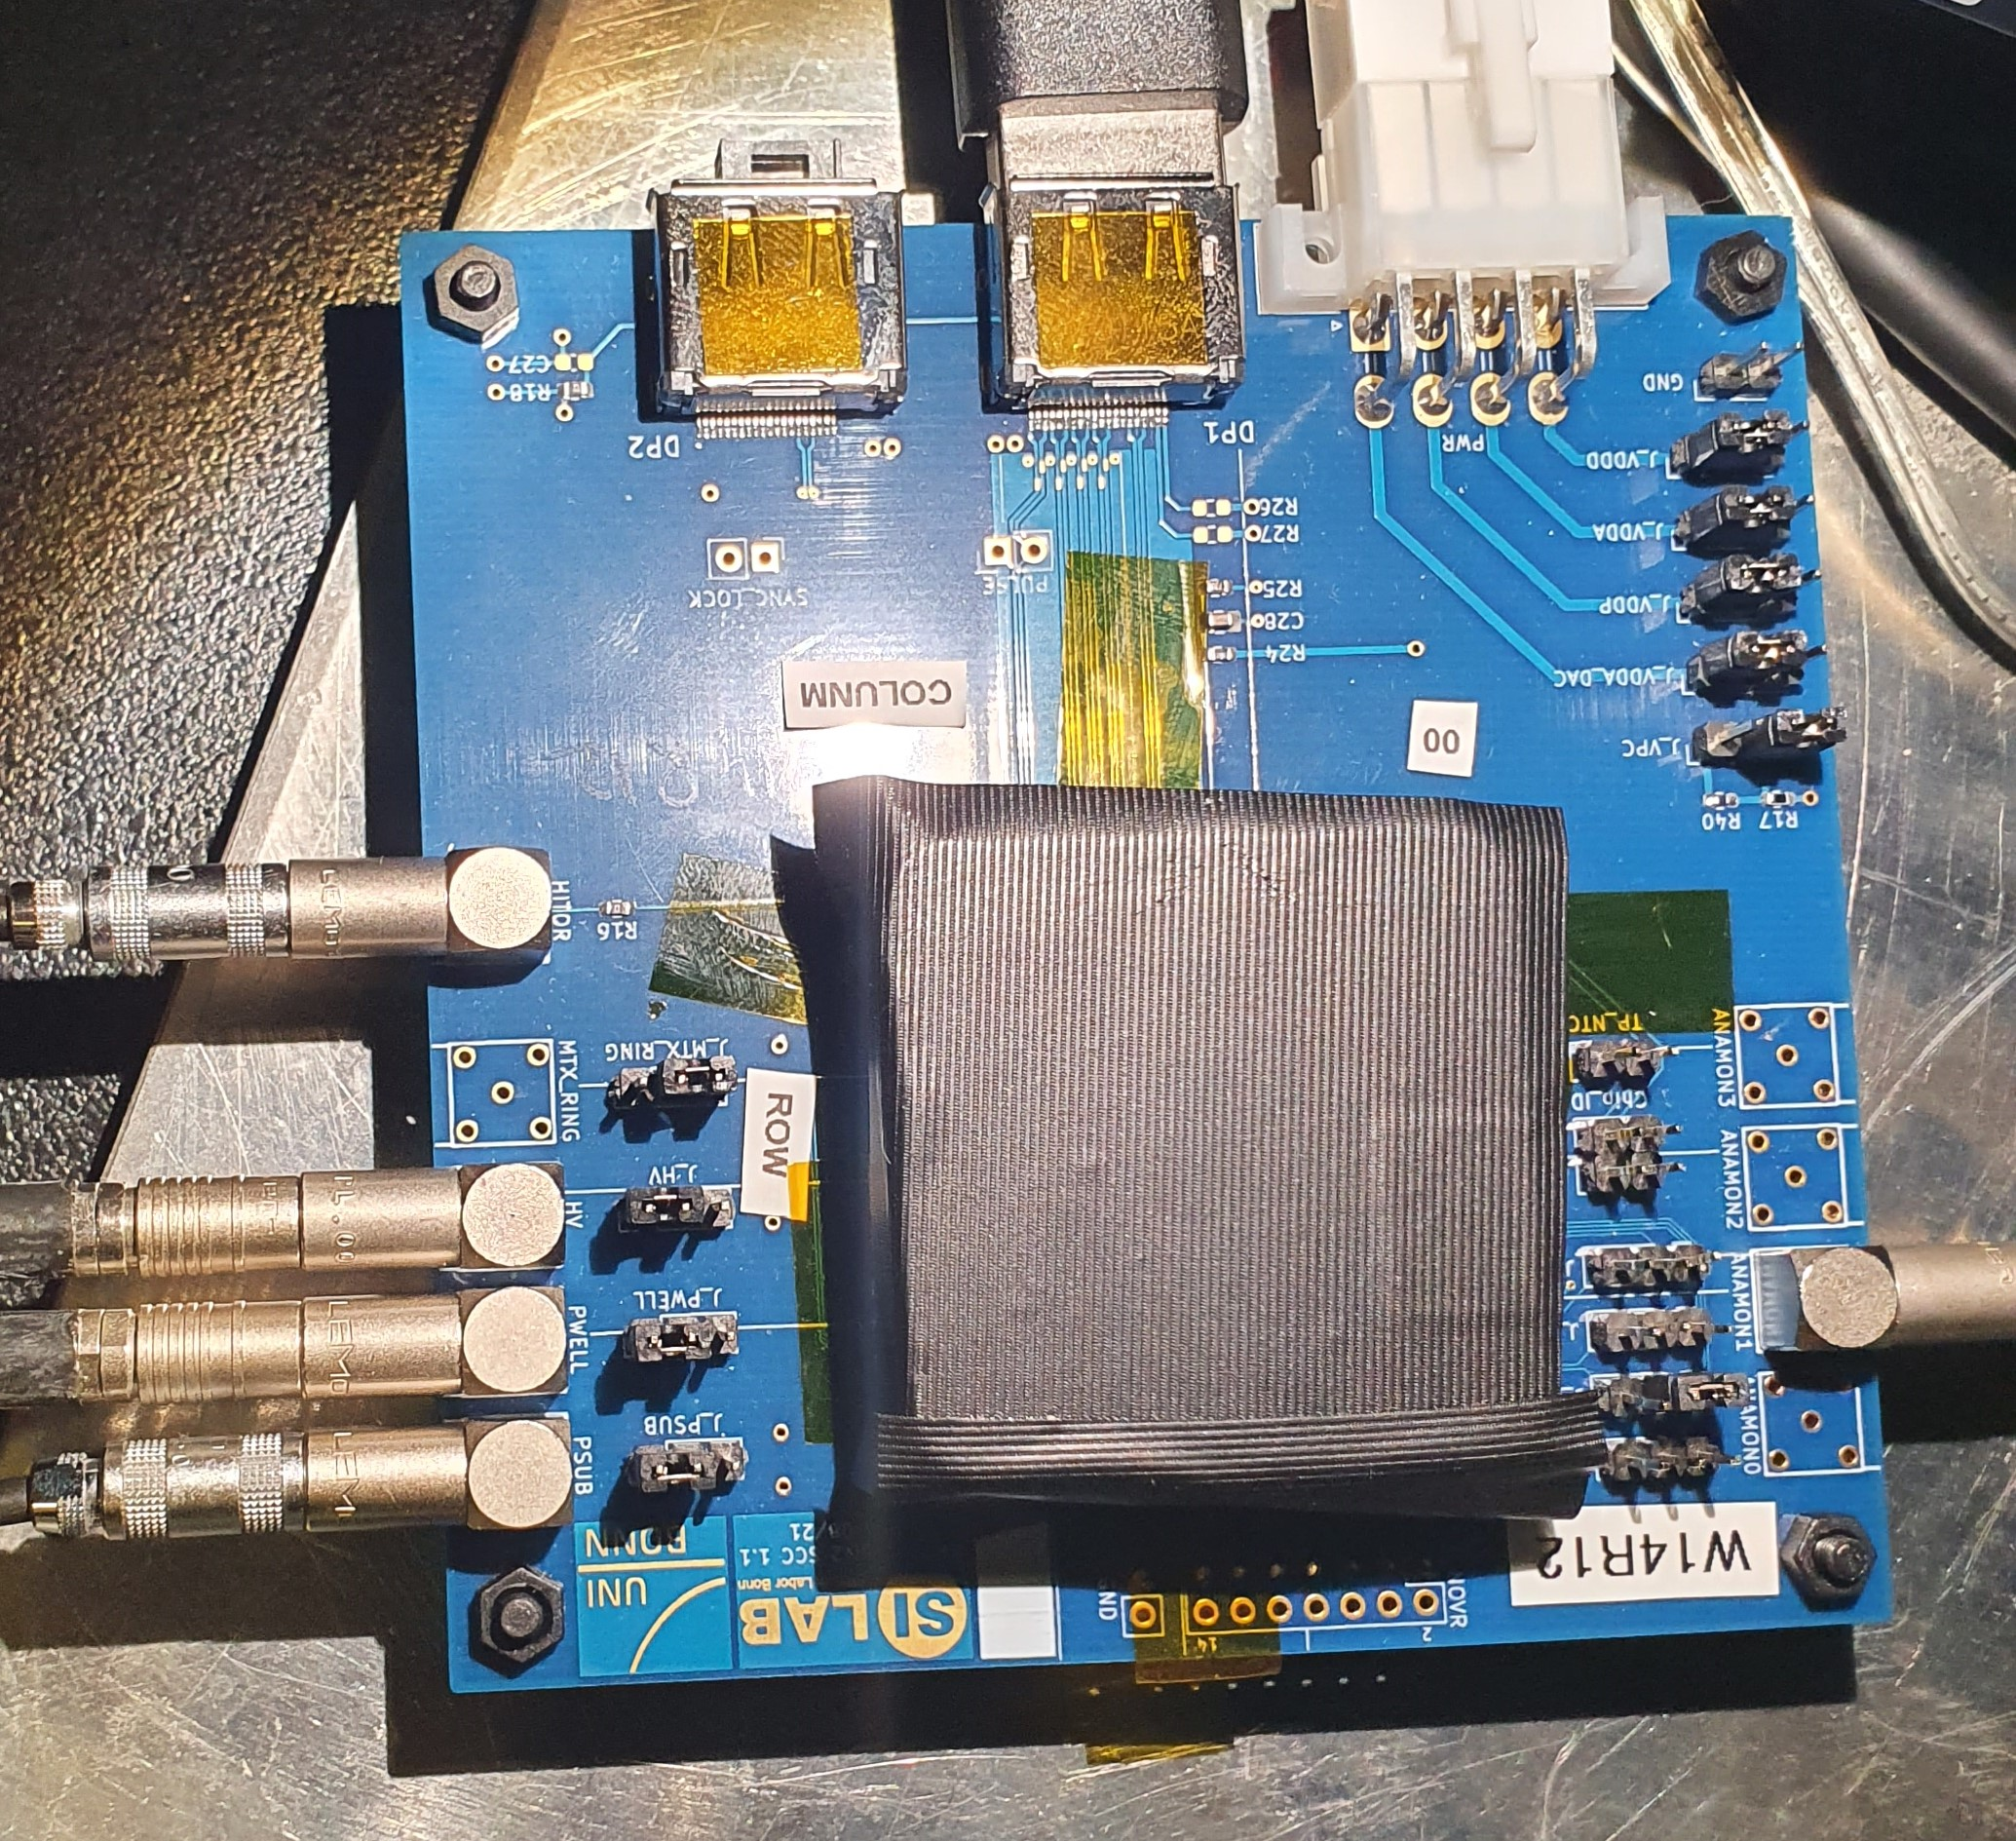
\includegraphics[scale=.08]{W14R12}
\caption{The W14R12 chip tested during the Test Beam in Desy.}
\label{fig:w14r12}
\end{figure}



% --------------------------------------------
%	5.1 MATRIX AND FLAVORS
%---------------------------------------------

\section{Matrix and flavors}

%DEVI SPIEGARE COSA è UGUALE A TJMONOPIX 1 SPIEGATO NEL QUARTO. QUI LE DIFFERENZE E LO STUDIO DELLE CARATTERISTICHE.
%%%RIFERIMENTO AL 4 SULLE implicazioni delle DIMENSIONI.

Tj-Monopix 2 is the next generation small collection electrode DMAPS prototype in TowerJazz 180 nm. The need to create a sensor capable to mantain high efficiency even after irradiation, required improvements compared to Tj-Monopix 1 in two important fields: a lower operating threshold and different pixel layout to increase charge collection efficiency all over its area, expecially in the corners.\\

To achieve these goals, a different front-end in pixel circuit was implemented and a lot of efforts have been focused on optimizing pixel layout in order to reduce its size which has been decreased to 33.04 x 33.04 $\mu m^{2}$. As a matter of fact we have seen in (REFERENCE) that pixel's dimensions are critical to accomplish faster charge collection across all active area, increasing the lateral electric field. For this reason it was necessary a special effort to design and create a smaller pixel but still adequate to embody the full digital readout. All of this required to work at the technology density limit and also for further modifications at the circuit design, such as single ended data transmission, in order to reduce the column-bus width.

%Aggiungi thickness 200um, pixel pitch 33.04um


%-----------------------------------------------------------------------------------------------%

\subsection{Flavors}

The protype is a 2 x 2 $cm^{2}$ pixel matrix which consists of 512x512 pixels and all of them are designed with a reduced deep p-well geometry (RDPW) because as it was demonstrated during the testing of TJ-Monopix1, this type of structure has a superior charge collection properties compared to full deep p-well coverage (FDPW) (figure \vref{fig:tj1pix_cov}). The total active area of the matrix is approximately 286 $mm^{2}$. 

\begin{figure}[h!]
\centering
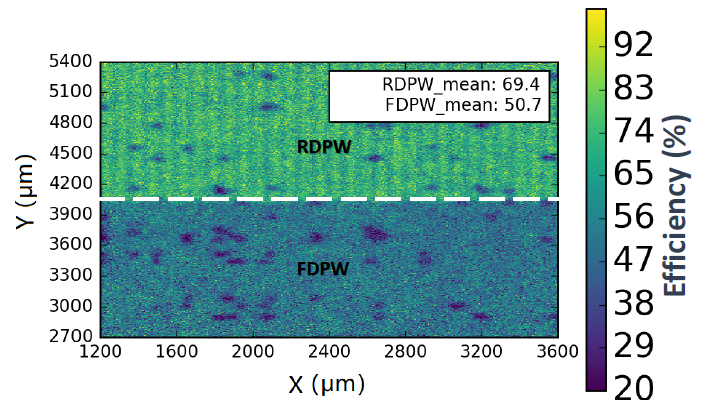
\includegraphics[scale=.6]{Tj1pix_cov}
\caption{Detection efficiency map of a TJ-Monopix1 chip with 25 $\mu$m p-epitaxial layer that has been irradiated to $10^{15}$ $n_{\textit{eq}}$/$cm^{2}$ NIEL.}
\label{fig:tj1pix_cov}
\end{figure}

As we can see in figure \vref{fig:tj2matrix}, the matrix is divided in four sectors, named \textbf{flavors} that implement different variation of the front-end circuit. In the first two flavors the collection electrode is DC-coupled directly with the readout electronics,  the continuous baseline reset is implemented by a forward bias diode and they differ for the pre-amplifier circuit design. The second flavor, named \textbf{Cascode FE}, includes an extra cascode transistor that increase the pre-amplifier gain and results in 50\% reduction of the threshold dispersion compared to the first flavor, the \textbf{Normal FE}. The other two flavors consist of AC-coupled pixels (through a metal-oxide-metal MOM capacitor) and in particular the \textbf{HV-Cascode FE} also incorporate the aforementioned pre-amplifier variation. AC-coupling allows to apply an high positive bias voltage (HV) to the collection electrode, but at the same time it also causes signal losses mainly due to the additional parasitic capacitance introduced at the sensitive input node.\\
The BCID bus width has been increased  to 7-bits due to higher gain and ToT slope with respect to Tj-Monopix 1. \\
It's worth mentioning here that the large column height (approx. 17 mm) due to large matrix area and the aggressive column-bus routing (which refers to the minimum line width and spacing) because of the smaller pixel size (always with respect to TJ-Monopix 1), generated a significant signal transmission delay due to the RC low pass filtering effect of the long metal wires. Consequently a special circuit has been studied that adds a variable delay to the hit pulse across the column that matches that of the BCID signal.


%%%PERIPHERY PAG 138


\begin{figure}[h!]
\centering
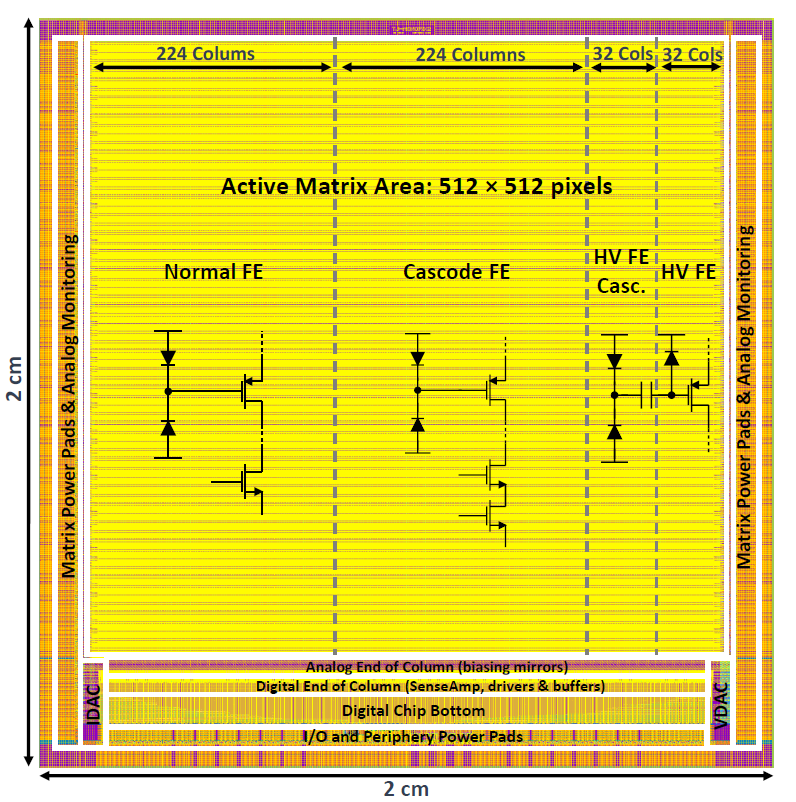
\includegraphics[scale=.5]{Matrix}
\caption{The layout of the TJ-Monopix2 prototype divided in four different flavors: \textbf{Normal}, \textbf{Cascode}, \textbf{HV-Cascode} and \textbf{HV FE}.}
\label{fig:tj2matrix}
\end{figure}


%-----------------------------------------------------------------------------------------------%

\subsection{Pixel design}

VEDI\\ 

The 2x2 pixel core layout, shown in figure \vref{fig:tj2core} is fully optimized and is designed in order to share as much functionality as possible between the four pixels. The analog area incorporates the front-end circuit, the 3-bit threshold tuning DAC and the pixel configuration registers. The digital region is composed by the 7-bit LE and TE memory (14 SRAM cells per pixel), the 10 bit address ROM (2 bit for the pixel position inside the core and 8 for the group address), the readout control logic and the hit delay circuit that is used to correct the BCID propagation delay. Two different token signals are used to set the priority of the pixels during the readout: the \textit{fast} one that propagates across the double column estabilished the priority between the cores and the \textit{local} one, which arbitrates the reading order of the four pixels inside each core.

\begin{figure}[h!]
\centering
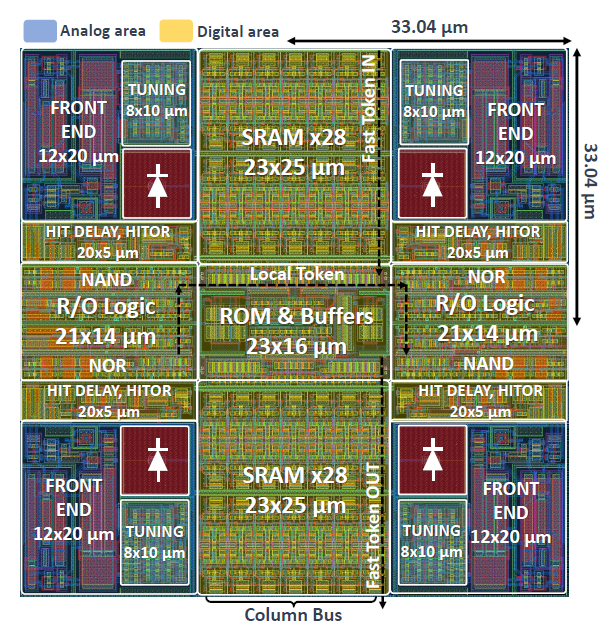
\includegraphics[scale=.5]{pixel_core}
\caption{Layout of a TJ-Monopix 2 2x2 pixel core. In blue the analog area and in yellow the digital one.}
\label{fig:tj2core}
\end{figure}


%-----------------------------------------------------------------------------------------------%

\subsubsection{Improved front-end circuit design}

As we have seen above, there are two variations of the front-end circuit,  ''normal'' and ''cascode'' type. The latter in particular includes an extra cascode transistor which increases the pre-amplifier gain and consequently reduces the threshold dispersion.\\
Moreover in TJ-Monopix 2 it was preferred to incorporate a simple diode to reset the input node instead of a PMOS transistor, which was the techonology implemented in TJ- Monopix 1. A side effect of this choice is that the relationship between charge injected and the ToT of the detected signal is not linear anymore, because the diode is a not linear element and its discharge rate also depends on the collected charge. Indeed in the following analysis it was necessary to fit the ToT trend with a more complex function. But at the same time, the advantages are its simplicity ($p^{+}$ diffusion within the n-well collection electrode) and also the fact that it allows to increase radiation tolerance to TID effects, which was one of the key working area in the upgrade of the sensor.

% in order to design a final(conclusive) prototype to employ in the experiments subjected to high radiation doses.[pag 153???] \\


In the last two AC-coupled flavors are implemented the same improvements, but here the different coupling provokes an important loss in the collected charge, as verified during the testing phase of TJ-Monopix 1 (50\% losses), due at most to additional parassitic capacitances. Thus a lot of efforts have been made to improve this aspect, working on the coupling capacitor values. A signal loss of 41.5\% has been reached, which is a relevant enhancement with respect to the predecessor.




% --------------------------------------------
%	5.2 THRESHOLD AND NOISE
%---------------------------------------------

\section{Threshold and noise}

In order to achieve the absolute calibration of the whole matrix, the response of each pixel has been characterize by means of the internal charge injection. \\

The hit injection circuit included in TJ-Monopix 2 is similar to the one of TJ-Monopix 1, shown in figure(????). It allows to inject artificial hits through an injection capacitance \textbf{$C_{inj}$} connected at the collection electrode, which is equal to 230 aF for both the DC and AC coupling FE. The injected charge is almost linear with the injection pulse amplitude (set by the two registers ''\textbf{$V_{L}$}'' and ''\textbf{$V_{H}$}'', like $\Delta V_{inj}$ = \textbf{$V_{H}-V_{L}$}). Moreover the injection step is finer compare to the one of TJ1 because of the higher voltage DAC resolution, in fact it is LSB (\textit{Least Significant Bit})=7.03 mV. The injected charge $Q_{inj}$ can be calculated from:

\begin{equation}
\small
Q_{inj} = \frac{230 \, aF}{q_{{e}^{-}}} \cdot \Delta V_{inj} = 1.4375 \frac{e^{-}}{mV} \cdot 7.03 \frac{mV}{DAC \, unit} \approx 10.1 \frac{e^{-}}{DAC \, unit}  
\label{conversion_factor}
\end{equation}

Eventually this value has been used to convert the information of the injected charge from DAC unit to electrons unit useful for further analysis.
\\
The four flavors have been separatly analyzed to be able to study their main difference concerning their performance and features, but the same method, called \textit{s-curve method} and explained below, has been used. 


%--------------------------------------------------------------------
\subsection{S-Curve method} \label{threshold_subsection}

In order to obtain the thresold and noise values for all pixels, each one of them has to be injected an arbitrary number of times (100 times in this work) for each value of the injection pulse between a minimum voltage value, chosen setting the chip register ''\textbf{VL}'' and a maximum volatge set by the ''\textbf{VH}'' register, with a step of 1 DAC unit (this is also adjustable). These two levels are provided by the voltage DAC.

So for each injection pulse height, the mean of 100 injection output are considered and it represents one data (marker) in the plot.  In this way, plotting the average number of detected hits in function of the injected charge, the typical curve better known as ''\textit{S-curve}'' is reconstructed. It can be fit with the \textit{Cumulative Distribution Function (CDF)}:

\begin{equation}
 CDF(Q) = \frac{1}{2} \cdot \bigg(1 + \textit{erf}\bigg(\frac{Q-\mu}{\sigma \sqrt{2}}\bigg)\bigg)
\end{equation}

from which the value of the threshold is evaluated considering the value of the injected charge at half of the curve's maximum height, so the parameter $\mu$ obtained from the fit and the noise is evaluated from the fit parameter $\sigma$. The ''\textit{erf(x)}'' is the Gauss error function. 

Specifically plotting the number of hits observed on each pixel divided by the total number of injections, for each injected charge, the half height corresponds to a charge value for which the pixel detects 50 hits of 100 injected and so when it has an occupancy of 0.5. In figure \vref{ex_scurve} is shown an example. \\

This method allows to study the noise and threshold of all pixels and also the threshold dispersion across an entire FE.

%%%%SPIEGARE METODO DI LUDOVICO???? 


\begin{figure}
\centering
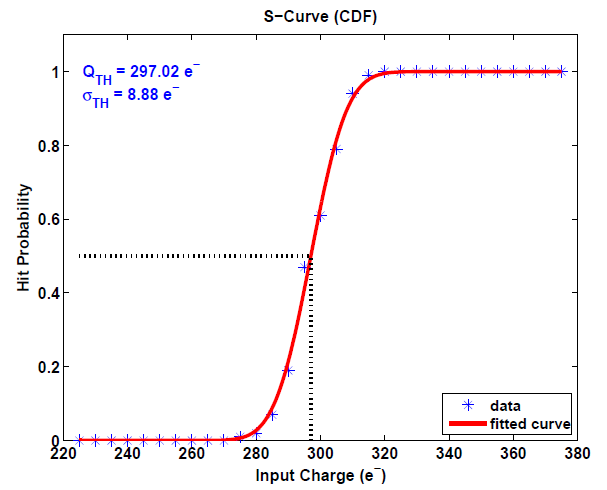
\includegraphics[scale=.6]{scurve_ex}
\caption{An example of the S-Curve fitted by the CDF to evaluate threshold and noise.}
\label{ex_scurve}
\end{figure}

In the following are reported the results of this study for the flavors of all matrix, injected a charge gradually increasing from 0 to 140 DAC ($\approx$ 1414 $e^{-}$ adopting the conversion factor in equation \ref{conversion_factor})


%THRESHOLD PATTERN EACH 32
%NOISE PATTERN UP DOWN

\subsubsection{Normal FE}

%PSUB/PWELL

The first flavor of the matrix is the \textbf{Normal FE}, which consist of 512 rows and 224 columns for a total of 114.688 pixels. The chip registers have been set with the same values used during the Test Beam at Desy (July 2022) which are different for the DC and AC-coupling case. They are known as ''\textbf{GOE settings}'' and they are reported in table \vref{tab:tb_settings}, where are also added the different biasing voltages used to power (up) the chip.

\begin{table}[h!]
\centering
\begin{tabular}{>{\columncolor{ProcessBlue!60}} C{3.2cm}|C{3.7cm}|C{3.5cm}}
\rowcolor{lightgray}
Registers & Normal/Cascode FE ($P_{SUB}$/$P_{WELL}$ = -3 V) & HV/HV-Cascode FE ($P_{SUB}$/$P_{WELL}$ = 0 V, HV = +5 V)\\[2ex]
\hline
$I_{THR}$ & 64 & 30\\[0.5ex]
\hline
$I_{BIAS}$ & 50 & 60\\
\hline
$V_{RESET}$ & 143 & 100\\
\hline
$I_{CASN}$ & 0 & 8\\
\hline
$V_{CASP}$ & 93 &40\\
\hline
$V_{CASC}$ & 228 & 228\\
\hline
$I_{DB}$ & 100 & 100\\
\hline
$I_{TUNE}$ & 53 & 53\\
\hline
$V_{CLIP}$ & 255 &255\\
\hline
$I_{COMP}$ & 80 & 80\\
\hline
$I_{DEL}$ & 88 & 88\\
\hline
$I_{RAM}$ & 50 & 50\\
\hline
\end{tabular}
\caption{Settings of the main registers used for all flavors (W14R12 chip) during the Test Beam in Desy.}
\label{tab:tb_settings}
\end{table}


\begin{figure}[h!]
\centering
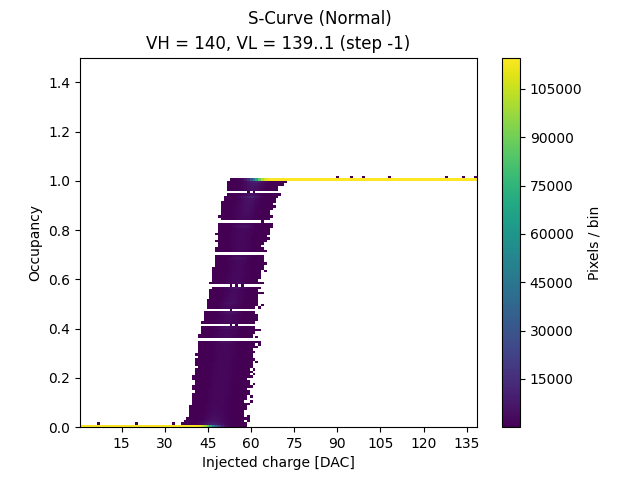
\includegraphics[scale=.6]{all_norm_thscan_140}
\caption{S-curves of all pixels of the Normal FE with an injection pulse of 140 DAC.}
\label{fig:norm_scurve_140}
\end{figure}

Using this setting, none of the pixels were noisy and so it wasn't necessary to use any mask.
In figure \vref{fig:norm_scurve_140} are plotted all the s-curves of the all well-functioning Normal flavor pixels. The width of the plot is a first indication (manifestation, symptom) of the threshold dispersion of the whole flavor.\\

The threshold and noise distributions obtained injecting all pixels as explained above, have been fitted with a gaussian distribution and they are shown in figure \pageref{fig:thdist_norm} with their maps, too.

\begin{figure}[h!]
\centering
\subfigure[Threshold distribution]
{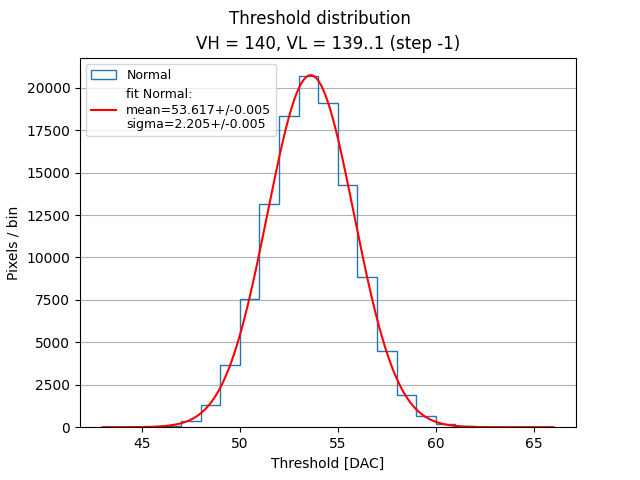
\includegraphics[scale=0.35]{all_norm_thdist_140}}\quad
\subfigure[Threshold map]
{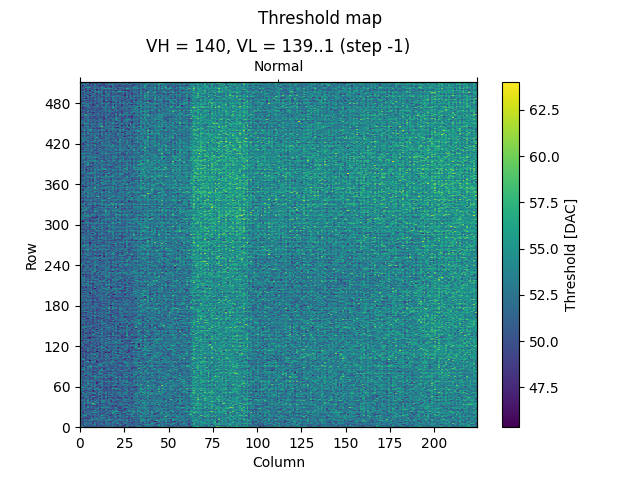
\includegraphics[scale=0.37]{threshold_map_norm_140}}\\
\subfigure[Noise distribution]
{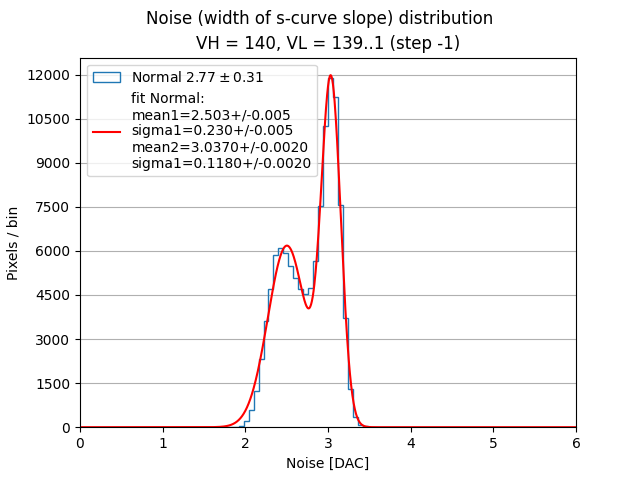
\includegraphics[scale=0.35]{Noise_hist_norm_140_fit}}\quad
\subfigure[Noise map]
{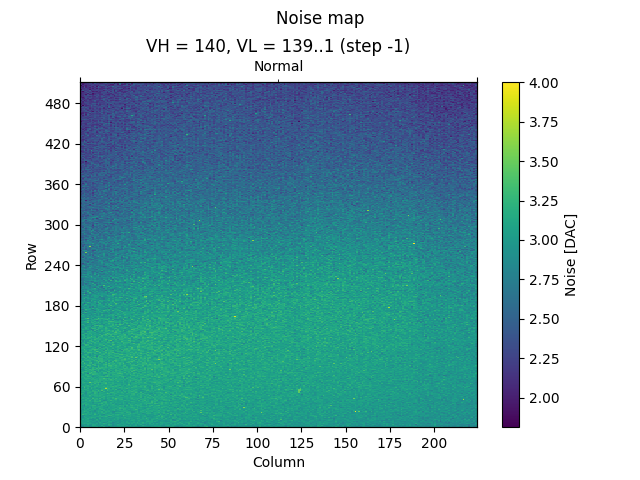
\includegraphics[scale=0.37]{Noise_map_norm_140}}\\
\caption{Normal FE.}
\label{fig:norm}
\end{figure}



\subsubsection{Cascode FE}

\textbf{Cascode FE} is the second flavor and like \textbf{Normal FE} it consists of 512 rows and 224 columns for a number of total pixels equal to 114.688. For this flavor the same procedure of Normale FE has been followed and also the same values' registers (table \vref{tab:tb_settings}) have been used. There were not find noisy pixels. 
In figure \vref{fig:casc_curve140} the S-curves of all pixels are shown.

\begin{figure}[h!]
\centering
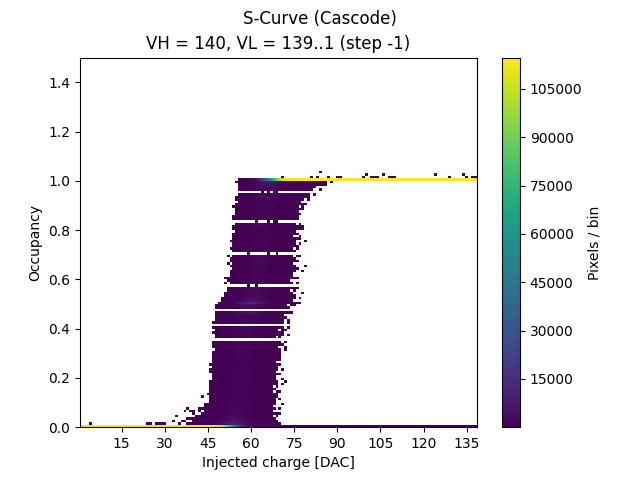
\includegraphics[scale=.5]{all_casc_thscan_140}
\caption{S-curves of all pixels in the \textbf{Cascode} flavor with an injection pulse of 140 DAC.}
\label{fig:casc_scurve140}
\end{figure}

The fit of the threshold and noise distributions and maps instead, are shown in figure \vref{fig:thdist_casc}.


\begin{figure}[h!]
\centering
\subfigure[Threshold distribution]
{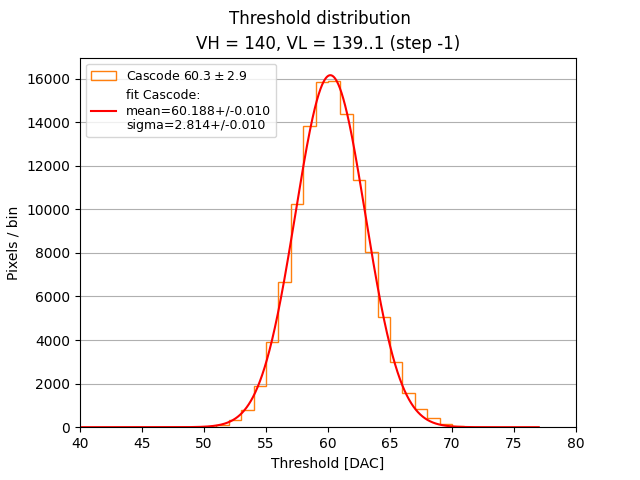
\includegraphics[scale=0.35]{all_casc_thdist_140}}\quad
\subfigure[Threshold map]
{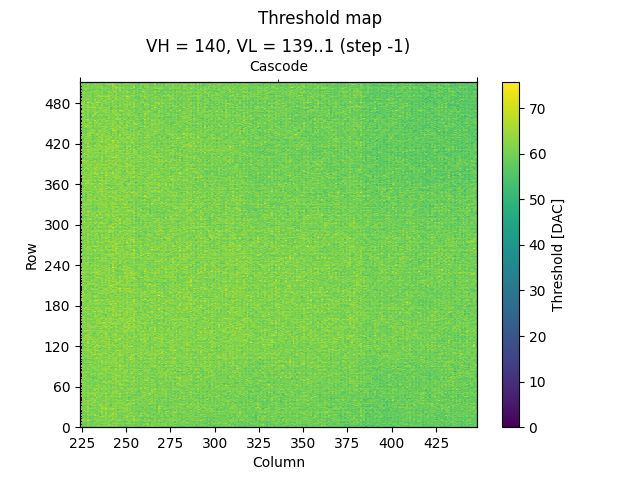
\includegraphics[scale=0.37]{threshold_map_casc_140}}\\
\subfigure[Noise distribution]
{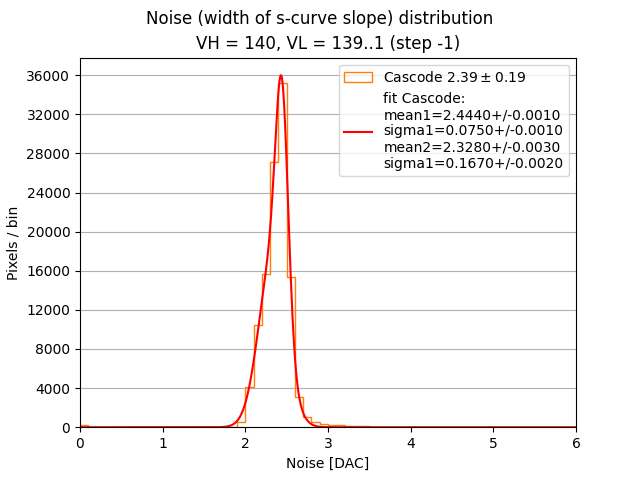
\includegraphics[scale=0.35]{Noise_hist_casc_140_fit}}\quad
\subfigure[Noise map]
{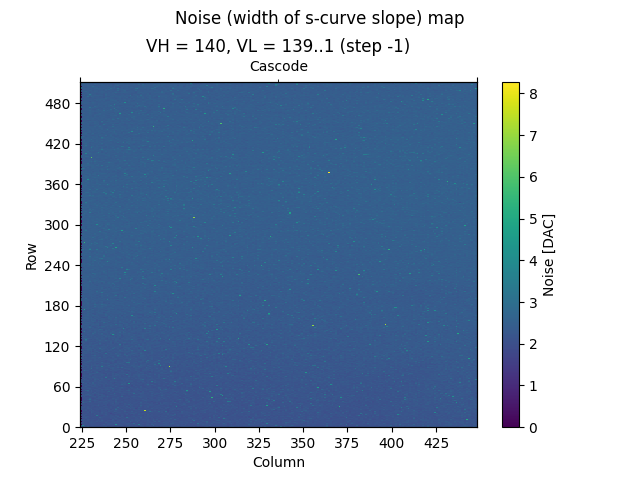
\includegraphics[scale=0.37]{Noise_map_casc_140}}\\
\caption{Cascode FE.}
\label{fig:norm}
\end{figure}

%%NO DIFFERENCE CUTTING NOISE >4 IN THE DISTRIBUTION. DIFFERENT FROM NORMAL



\subsubsection{HV-Cascode FE}

%PSUB/PWELL

The third flavor is \textbf{HV-Cascode FE} where HV stands for \textbf{High Voltage} and it is formed (counts) of 512 rows and 32 columns for a total number of pixel equal to 16384. Also for these last two flavors, the main chip registers are set with the same values tested and used during the Test Beam (@Desy) (but different from those used for the first two flavors). They are reported in table \vpageref{tab:tb_hv_settings} .

As we can see from the plot of the alle S-curves in figure \vpageref{fig:hvc_scurve_140}, there were a lot of noisy pixels with these choices of values' registers, but at this stage of measurements they were not masked.
As a matter of fact along the y-axis of this plot is displayed the occupancy and when this values becomes higher than 1, it means that the pixel detects more hits than the injected ones, so it could be identified as ''\textit{noisy pixel} (because it results active regardless of the charge injection)''.


\begin{figure}[h!]
\centering
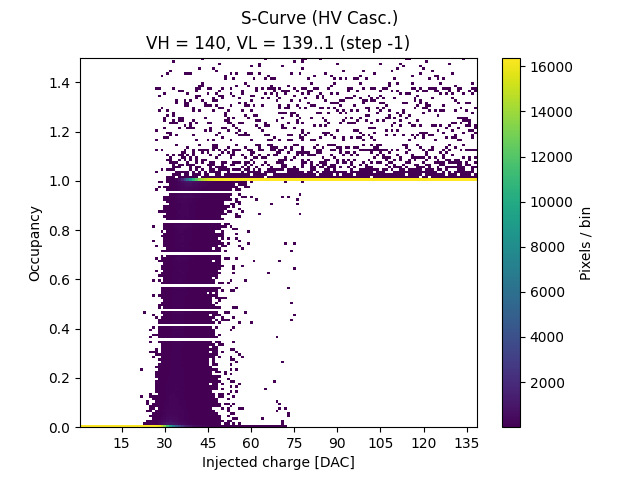
\includegraphics[scale=.5]{all_HVc_thscan_140}
\caption{S-curves of all pixels in \textbf{HV Cascode} flavor with an injection pulse of 140 DAC.}
\label{fig:hvc_scurve_140}
\end{figure}

In figure \vref{fig:thdist_hvc} are shown the fit of the threshold and noise distributions.

\begin{figure}[h!]
\centering
\subfigure[Threshold distribution]
{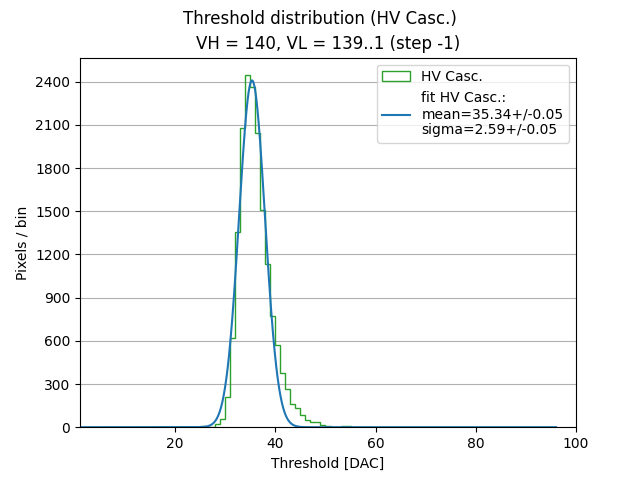
\includegraphics[scale=0.35]{all_HVc_thdist_140}}\quad
\subfigure[Noise distribution]
{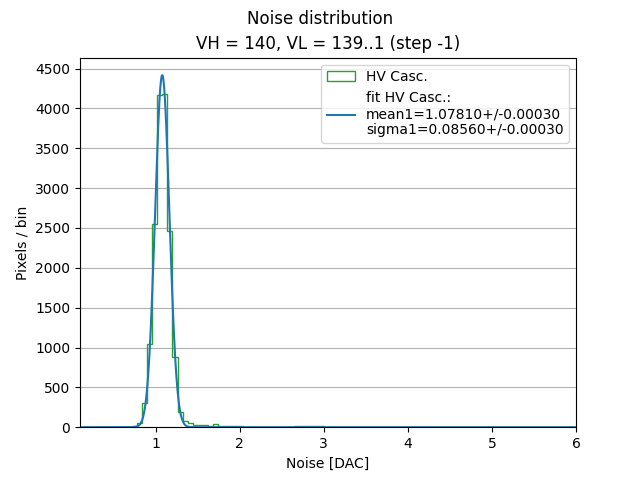
\includegraphics[scale=0.37]{Noise_hist_HV Casc._140_fit}}\\
\caption{HV Cascode FE.}
\label{fig:thdist_hvc}
\end{figure}


\subsubsection{HV-Normal FE}

The fourth and last flavor is the \textbf{HV-Normal FE} which consists of 512 rows and 32 columns for a total number of pixel equal to 16.384. The main registers have been set with the values reported in table \vpageref{tab:tb_hv_settings}.
In figure \vpageref{fig:hv_scurve_140}, the S-curves of all pixel in the flavor. Also here we can see that there were some noisy pixels unmasked.
Moreover, in this final flavor, the last 16 columns were not working (visible in the maps in figure \vpageref{HVs_maps}) and as a matter of fact they had return a peak of threshold near the value 0, which is excluded from the threshold distributions plots.

So actually in this part of the matrix, the real number of pixel studied was the half of the total, such as 8192 pixels.


\begin{figure}[h!]
\centering
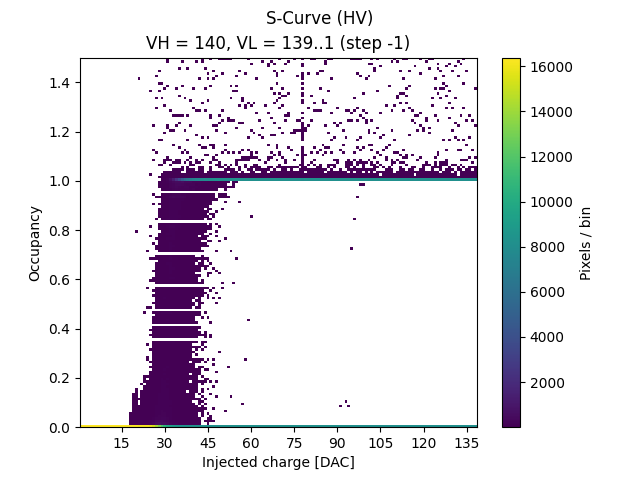
\includegraphics[scale=.5]{all_HV_thscan_140}
\caption{S-curves of all pixels in \textbf{HV Cascode FE} with an injection pulse of 140 DAC.}
\label{fig:hv_scurve_140}
\end{figure}

In figure \vref{fig:thdist_hv} the fit of the threshold and noise distributions.

\begin{figure}[h!]
\centering
\subfigure[Threshold distribution]
{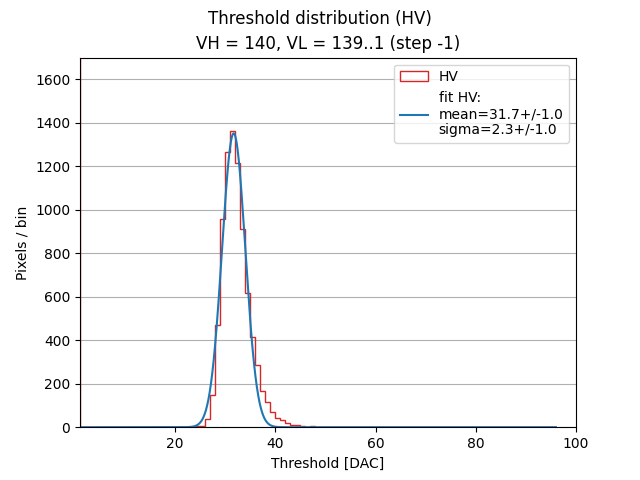
\includegraphics[scale=0.35]{all_HV_thdist_140}}\quad
\subfigure[Noise distribution]
{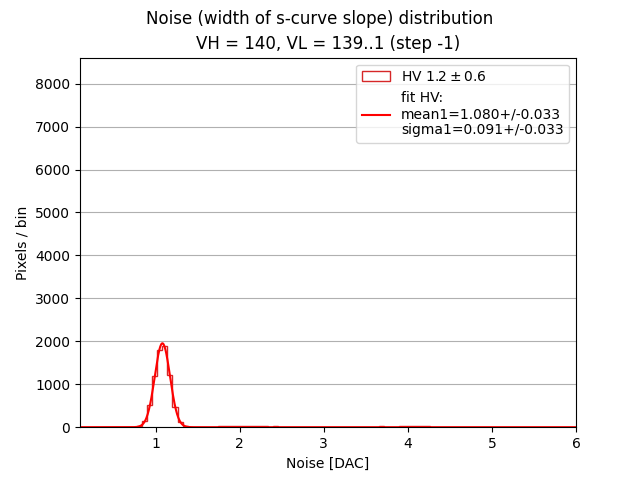
\includegraphics[scale=0.37]{Noise_hist_HV_140_fit}}\\
\caption{HV Normal FE.}
\label{fig:thdist_hv}
\end{figure}


At last in figure \vpageref{HVs_maps} the threshold and noise maps of the whole HV flavor.

\begin{figure}[h!]
\centering
\subfigure[Threshold map]
{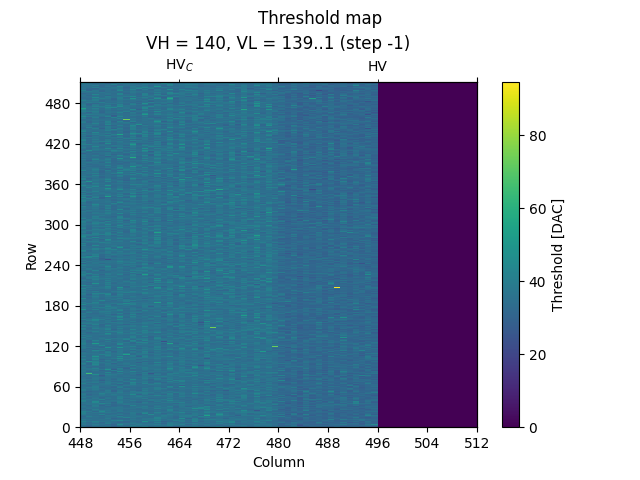
\includegraphics[scale=0.35]{threshold_map_All FEs_140}}\quad
\subfigure[Noise map]
{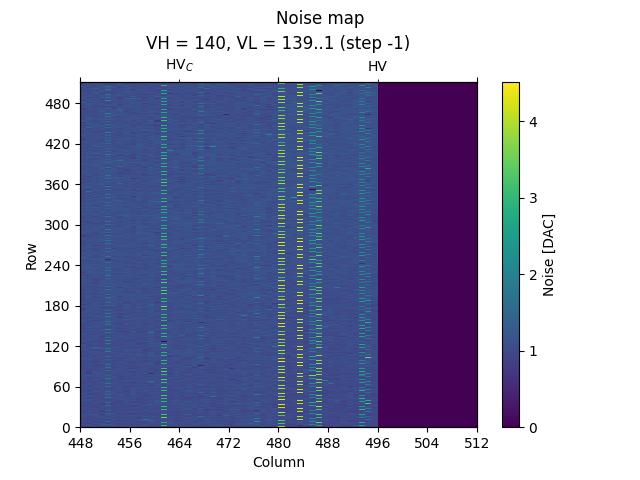
\includegraphics[scale=0.37]{Noise_map_HV Casc._140}}\\
\caption{HV's FE.}
\label{fig:HVs_maps}
\end{figure}

As we will see in the following (section REFERENCE), the atypical s-curves in HVs flavors have been the first hint(evidence) of the cross-talk problem (section REFERENCE) tied to a lower global threshold in these sectors with TB settings. 


\subsubsection{Summary Table}

In table \vpageref{th_noise_all} a summary of results for threshold, noise and threshold dispersion of all FE.

\begin{table}[h!]
\centering
\begin{tabular}{>{\columncolor{NavyBlue!70}} c|c|c|c}
\rowcolor{CornflowerBlue}
Front-End & Threshold [$e^{-}$] & Threshold dispersion [$e^{-}$] & Noise [$e^{-}$]\\
\hline
Normal  & 53.62 $\pm$ 0.01 & 2.21 $\pm$ 0.01 & \shortstack{2.503 $\pm$ 0.005 \\ 3.037 $\pm$ 0.002}\\
\hline
Cascode & 60.19 $\pm$ 0.01 & 2.81 $\pm$ 0.01 & 2.400 $\pm$ 0.003\\
\hline
HV - Cascode & 35.34 $\pm$ 0.05 & 2.59 $\pm$ 0.05 & 1.0781 $\pm$ 0.0003\\
\hline
HV & 31.70 $\pm$ 0.10 & 2.30 $\pm$ 0.10 & 1.080 $\pm$ 0.033\\
\hline
\end{tabular}
\caption{Summary table of threshold and noise values for all flavors of the W14R12 chip.}
\label{tab:th_noise_all}
\end{table}



%--------------------------------------------------------------------
\subsection{Threshold dispersion and tuning}

%CITAZIONE 8BIT BIASING DAC NEL PRECEDENTE???

Despite its predecessor, Tj-Monopix 2 is equipped with a circuit which allows the \textit{threshold tuning}. In other words it can adjust every pixel threshold, even if only by few DAC, in order to have a global threshold on the matrix as uniform as possible, or in any case a dispersion as small as possible, expecially after irradiation. We have already noticed that ( took a look to) (\vref{fig:tj2core}) the analog part of the in-pixel front-end that includes the 3-bit threshold tuning DAC, which not only improves the global threshold dispersion across the pixels, but also solves the issue with the unintentionally masked ghost pixels, reducing the noise even more. This system has been design in order to decrease the some effects that affected the threshold disperision like systemstics (for example, related to biasing), process and temperature variations and radiation damage. \\

Threshold trimming of each (individual) pixel is performed with the help of a tuning DAC (TDAC), shown in figure \vref{fig:tdac}. In particular this component controls the discriminator active load (comparison?) current $I_{DISC}$ which is partly(?) responsible of the pixel threshold. It works as an analog multiplexer (consisting of simple PMOS transistor switches), which selects one of seven $I_{DISC, n}$ lines generated by the main 8-bit biasing DAC. So the possbile vaue of the final $I_{DISC}$ is given by the sum of two contributions:

\begin{equation}
I_{DISC} = I_{DISC, coarse} + (TCODE - 1) \cdot I_{DISC,fine},  \hspace{.5cm}	where \hspace{.5cm} 1 \leq TDAC \leq 7
\end{equation}

\textbf{$I_{DISC, coarse}$} is the current sets by the main(raw?) value of threshold, resulting by the setting of the main registers which are responsible for it. 
\textbf{$I_{DISC, fine}$} is the current selected by the fine tuning step (TDAC) and it depends on the 3-bit tunning code that is stored in the in-pixel tuning memory latch (the in-pixel configuration memoty).
\textbf{TCODE} is the decimal representation of the TDAC code. 

For example if the 3-bit DAC are set to ''111'', the decimal representation is 8 and the fine tuning provide a current $I_{DISC,7}$, which corresponds to the highest threshold. If the 3-bit are set to ''010'' the corresponding TCODE is 2 and the current $I_{DISC,1}$ is provided that set the lowest threshold possible around the central value $I_{DISC,coarse}$. The particular combnation ''000'' instead (TCODE = 0) masks the pixel by disabling the discriminator, without affects the functioning(operation) of the others.

\begin{figure}
\centering
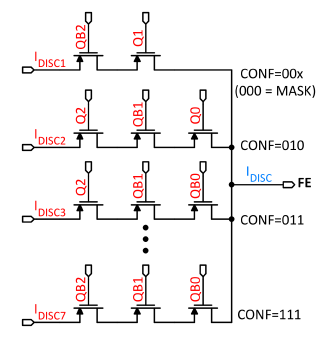
\includegraphics[scale=.8]{tuning_b}
\caption{Schematic of 3-bit tuning DAC (TDAC)}
\label{fig:tdac}
\end{figure}

%MA COME AGISCE IDISC: 19.10 LOGBOOK increasing TDAC/IDISC, lower threshold

\subsubsection{Results from fine tuning}

It has been trying to apply the fine tuning method to level out the threshold of some pixels as much as possible. \\

Results from measurements done later (Ludovico talk TREDI) pre and post



%--------------------------------------------------------------------
\section{ToT calibration with internal injection}

%%SIGLA TOT per la prima volta devi aggiungere, come anche PMOS .

%TOT VS Q_INJ CALIBRATION CURVE

As it has been pointed out in the previous, choosing to use a simple diode instead a PMOS transistor as reset input baseline element, increases the tolerance to TID radiation but at the same time it implicates a non-linear relationship between the injected charge and the ToT.  For this reason, one of the target of this analysis consisted to fit the trend (?) $Q_{inj}$ vs. ToT, in order to obtain the absolute calibration of the whole matrix.


%--------------------------------------------------------------------
\subsection{Injection circuit issues} \label{inj_issue}

%SATURATION INJECTION CIRCUIT

In carrying out the measurements mentioned above, we started to noticed some issues with the injection circuit, which seemed to limit its working range. As a matter of fact the height of the injection pulse is expected to grow linearly increasing the value of charge to be injected.
It actually happened up to a value of (about) $\approx$ 140 DAC, but for higher quantities of injected charge, the circuit seemed to increase not only the height of the signal, but also the threshold by a certain amount of $\Delta V$ (or equivalently of $\Delta Q$, related by the conversion factor reported in REFERENCE). Moreover, for injection height grater than 200 DAC, only the threshold grows, without increasing the actual injected charge in any way.\\
We come to the conclusion that the grows of the threshold was artificial and due to the failure of the injection circuit.[?]

However as we have seen in the previous section (reference), the threshold depends on the settings of the chip registers and it can't be influenced by the injected charge, otherwise the whole response of the chip would be chaotic and it would not be reliable to take precise measurement of the impinging particles. \\

A method (recipe) has been therefore devised to obtain a reliable values of threshold and ToT up to a value of 170 DAC of effective (actual) charge injected. Moreover the characterization of the function to describe the $Q_{inj}$ - ToT relationship has allowed also to extrapolated ToT values in the forbidden region of charge by the internal injection circuit issue (above $\approx$ 1717 $e^{-}$), that usually corresponds to the emission peaks of the radioactive sources available in the laboratory.


%--------------------------------------------------------------------
\subsection{Time Over Threshold (TOT) curves and fit} \label{tot_fit}

The function chosen for this purpose is:

\begin{equation}
y(x) = a\cdot x +b -\frac{c}{x-t}
\label{fit_function}
\end{equation}

with \textit{a}, \textit{b}, \textit{c} and \textit{t} free parameters and where the \textit{y} represents the ToT corresponding to a precise value of collected charge, express by \textit{x}. 

Actually we know that the ToT distribution starts to grow near the threshold, so a random parameter among them, could be computed in function of the threshold value estimated from the previous measurements, explained (shown, described) in section \ref{threshold_subsection}.

In particular knowing that y($x_{th}$) must be equal to 0, that is the ToT at the value of the threshold, it can be imposed:

\begin{equation}
0 = a\cdot x_{th} + b - \frac{c}{x_{th}-t}  \hspace{.4cm}	\Rightarrow  \hspace{.4cm}	c = x_{th}^{2}\cdot a + x_{th}\cdot (b-a\cdot t) - t\cdot b
\end{equation}

In this way the number of parameters to fit is reduced.

So the same data collected in the previous measurements of thresholds have been used to fit the ToT curves of all pixels for each frontend, so the registers are set in according to the ''GOE'' settings (\vref{tab:tb_settings} for Normal and Cascode FE and \vref{tab:tb_hv_settings} for HV's).
In table \vref{tab:th_fe} are reported the value of the threshold considered for each one of them (so that) to extrapolate the value of the parameter \textit{c} and the results of the fit for all parameters. In figure \vref{fig:tot_fe} the results obtained for all Normal, Cascode and HVs FE. The parameter \textit{c} is chosen only for simplicity of calculation.

\begin{table}[h!]
\centering
\begin{tabular}{c|c|c|c|c}
 & \textbf{Normal} & \textbf{Cascode} & \textbf{HV Cascode} & \textbf{HV} \\
\hline
\textit{threshold [DAC unit]} & 53.62 & 60.19 & 35.34 & 31.70 \\
\textit{a} & & & & \\
\textit{b} & & & & \\
\textit{c} & & & & \\
\textit{t} & & & & \\
\end{tabular}
\caption{Threshold and parameters obtained from the fit of ToT curve for each frontend.}
\label{tab:th_fe}
\end{table}

\begin{figure}[h!]
\centering
\subfigure[\textbf{Normal}]
{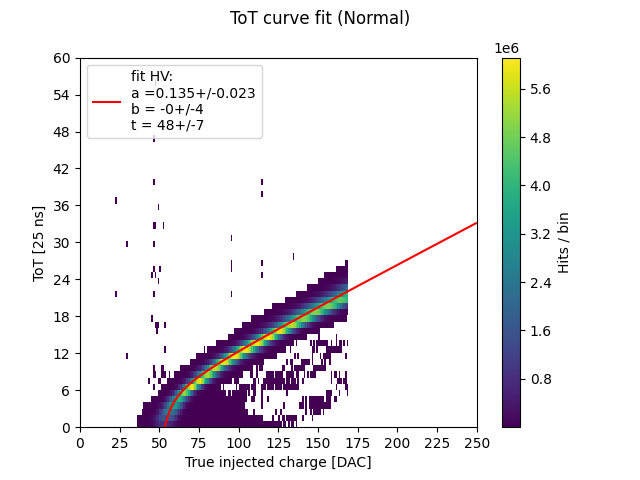
\includegraphics[scale=0.35]{tot_fit_normal(200)}}\quad
\subfigure[\textbf{Cascode}]
{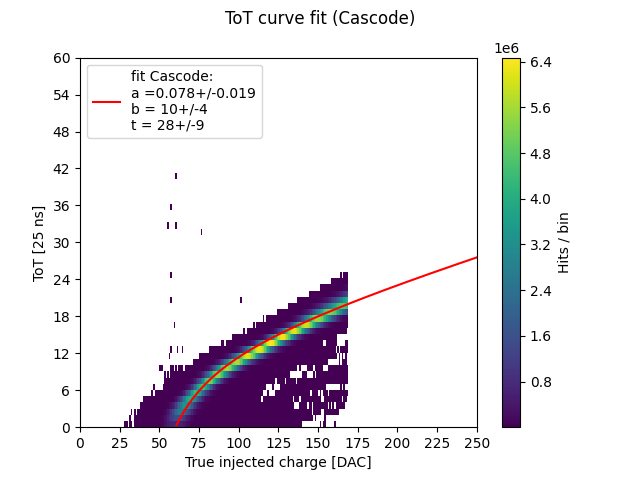
\includegraphics[scale=0.35]{tot_fit_cascode(200)}}\\
\subfigure[\textbf{HV Cascode}]
{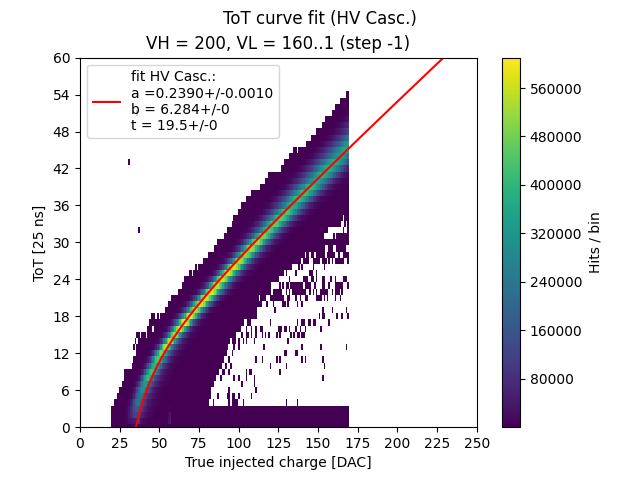
\includegraphics[scale=0.35]{tot_fit_HV_Casc.(200)}}\quad
\subfigure[\textbf{HV}]
{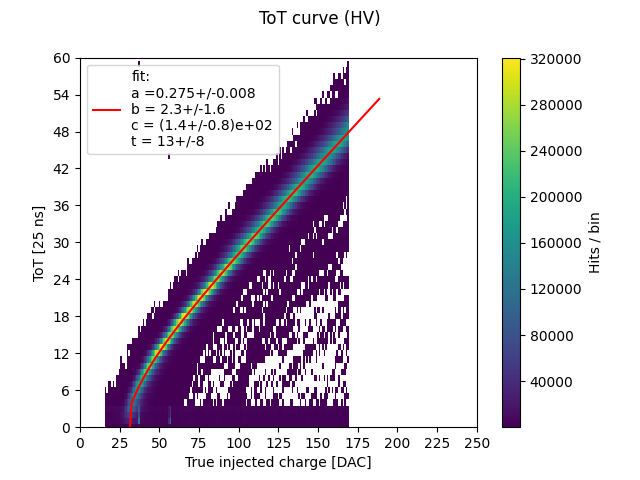
\includegraphics[scale=0.35]{tot_fit_HV(200)}}\\
\caption{ToT curves fit for all frontend.}
\label{fig:tot_fe}
\end{figure}


%--------------------------------------------------------------------
\section{Response to radioactive source and absolute calibration} \label{source_ana}

%06/10/2022 LOGBOOK

The absolute calibration of the matrix consists in characterizing the signal response (conversion gain?) of pixels for each FE. By the means of the $Q_{inj}$ - ToT fit (section \ref{tot_fit}), it is posible to extrapolate (deduce, estimate) the value of the ToT of the signal induced for whatever collected charge. At this point then, three (or four) different X-rays radioactive sources were used to study the signal spectrum and the response time of the matrix, with emission lines from 6 to 60 KeV (1600 to 16000 e-).??? 
In fact the known energies of the sources emission spectrum (so that the charge released in the matrix from particles emitted in decays) allow to compare the spectra obtained irradiating the chip, with the expected value of their peaks. [Only the events in which all charge inducted is collected in a single pixel are a part of the peaks reconstructed by the chip.]\\
Moreover these radioactive sources allowed to extend the ToT calibration for(at) higher value with respect to the limit imposed by the saturation of the internal injection circuit (section \ref{inj_issue}). In table \vref{tab:radio_sources} are shown the emission energies of the sources employed, that it was possible to see with the chip under test.

[Considering that the average energy necessary to produce an electron/hole pair in silicon is 3.65 eV, it is possible to convert the peak energies in a mean value of electrons released by the means of equation \vpageref{energy_electron_conv}. So in the table are reported also the equivalent emission in electrons, which will be useful further.]

\begin{equation}
N_{e^{-}} = \frac{E \, [eV]}{3.65 [\frac{eV}{e/h \, pair}]}
\label{energy_electron_conv}
\end{equation}
%%CONVERSIONE IN ELETTRONI
%SR90 BETA SOURCE???


\begin{table}[h!]
\centering
\begin{tabular}{>{\columncolor{NavyBlue!70}} C{3cm}|C{2.8cm}|C{2.8cm}}
\rowcolor{CornflowerBlue}
Source & Energy $\gamma$ [KeV] & Equivalent charge [$e^{-}$]\\[2ex]
\hline
\ch{^{55}Fe} & 5.9 & 1616\\[0.5ex]
\hline
\ch{^{241}Am} & 13.9 & 3808\\[0.5ex]
\hline
\ch{^{241}Am} & 17.7 & 4849\\[0.5ex]
\hline
\ch{^{241}Am} & 20.7 & 5671\\[0.5ex]
\hline
\ch{^{109}Cd} & 22 & 6027\\[0.5ex]
\hline
\ch{^{241}Am} & 26.4 & 7233\\[0.5ex]
\hline
\ch{^{241}Am} & 59.7 & 16356\\
\hline
\end{tabular}
\caption{Emission lines of \ch{^{55}Fe}, \ch{^{241}Am}, \ch{^{109}Cd} sources visible by the sensor.}
\label{tab:radio_sources}
\end{table}

%--------------------------------------------------------------------
\subsection{\ch{^{55}Fe}}

The \ch{^{55}Fe} source decays by \textbf{electron capture} to \ch{^{55}Mn}. One of the photons emitted in this transistion has an energy of 5.9 KeV ($K_{\alpha}$) and it produces in turn a photo-electron which deposits a inization charge of about 1616 $e^{-}$ in the sensor. 
All flavors were irradiate with a \ch{^{55}Fe} source available in the laboratory (scrivi caratteristiche). In figure \vref{fig:fe_all} are shown the results obtianed. Each peak were fitted by a gaussian function, limited in the region of the peak itself. The hump (shoulder, bump) for smaller ToT is a consequence of charge sharing among pixels. 

\begin{figure}[h!]
\centering
\subfigure[\textbf{Normal}]
{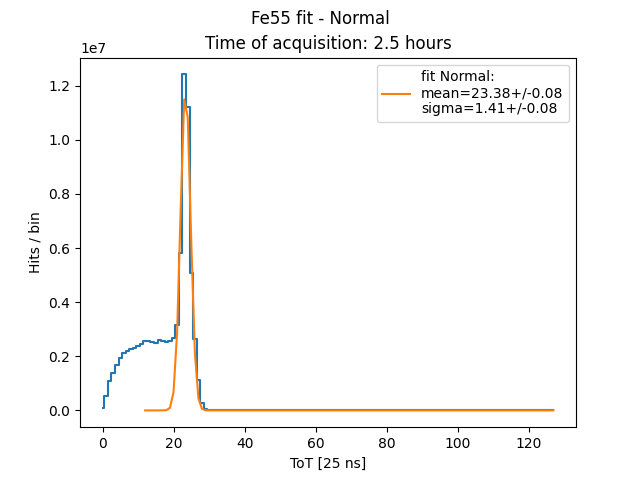
\includegraphics[scale=0.35]{fe55_Normal_peak}}\quad
\subfigure[\textbf{Cascode}]
{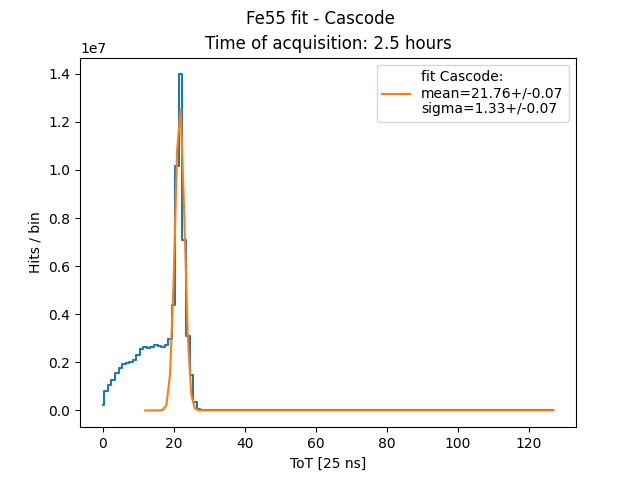
\includegraphics[scale=0.35]{fe55_Cascode_peak}}\\
\subfigure[\textbf{HV Cascode}]
{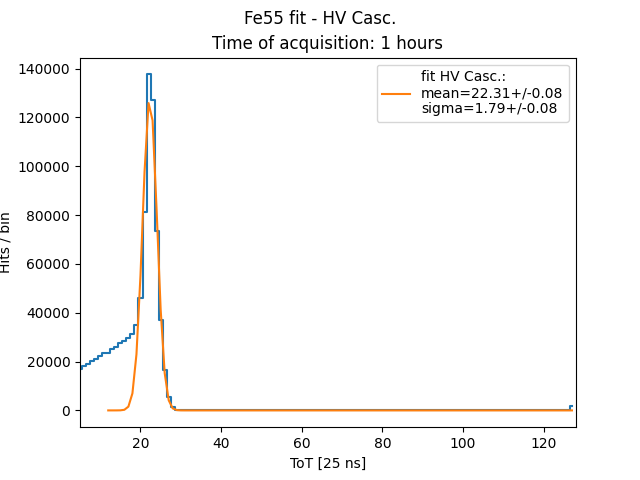
\includegraphics[scale=0.35]{fe_HV Casc._peak}}\quad
\subfigure[\textbf{HV}]
{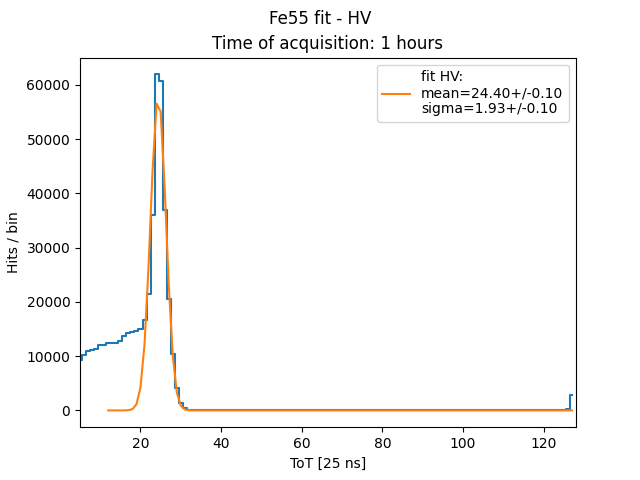
\includegraphics[scale=0.35]{fe_HV_peak}}\\
\caption{\ch{^{55}Fe} peaks for all frontends.}
\label{fig:fe_all}
\end{figure}

As it can be seen for the HV's FE a cut has been applied only to make clearly visible the emission line beacuse a lot of noisy pixels caused a sharp peak at 0 ToT. As a matter of fact in this flavors there were several column of not-functioning pixels. In the box of each plot are also reported the results of the fit that will be crucial in the following.


%--------------------------------------------------------------------
\subsection{\ch{^{241}Am}}

%AGGIUNGI REFERENZA IMMAGINE (Measurements of gamma-ray emission probabilities of 241, 243Am and 239Np)
%AGGIUNGI REFERENZA (GAMMA RAY SPECTRUM OF AM-241 IN A BACK SCATTERINGGEOMETRY USING A HIGH PURITY GERMANIUM DETECTOR)

The \ch{^{241}Am} source has a more complex spectrum (figure \vref{fig:am241_spectrum}) and not all its peaks can be revealed (detected) by the chip (because of the limited range of ToT available, depending on the bit dedicated to it). The spectrum shows other minor peaks besides the usual intense gamma peaks (59.5 and 26.3 keV) and several characteristic L X-rays from \ch{^{237}Np} (20.7, 17.7 and 13.9 keV).\\ 
Results are reported in figure \vref{fig:am_all}. In the case of the first two flavors, it could be possible to fit four peaks of the emission lines. In case of the HV's flavors instead, only three peaks for the HV-Cascode FE and two for the HV. As a matter of fact the AC-copuling causes about 41\% of signal loss (reference), so they are much less evident and more difficult to fit as isolated peak.

\begin{figure}[h!]
\centering
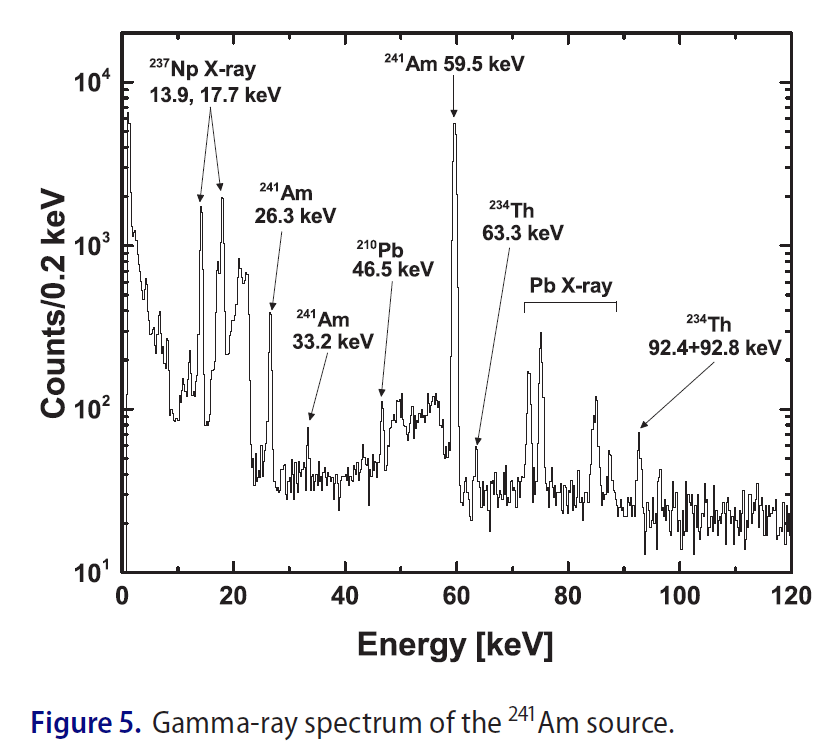
\includegraphics[scale=.4]{Am241}
\caption{\ch{^{241}Am} $\gamma$ emission spectrum.}
\label{fig:am241_spectrum}
\end{figure}


\begin{figure}[h!]
\centering
\subfigure[\textbf{Normal}]
{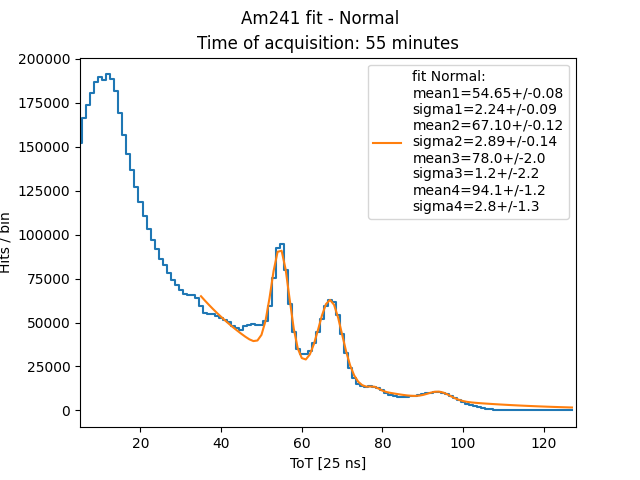
\includegraphics[scale=0.35]{am_Normal_peak}}\quad
\subfigure[\textbf{Cascode}]
{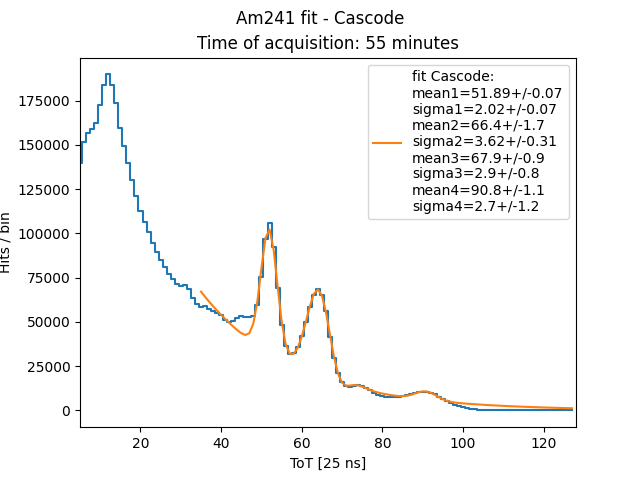
\includegraphics[scale=0.35]{am_Cascode_peak}}\\
\subfigure[\textbf{HV Cascode}]
{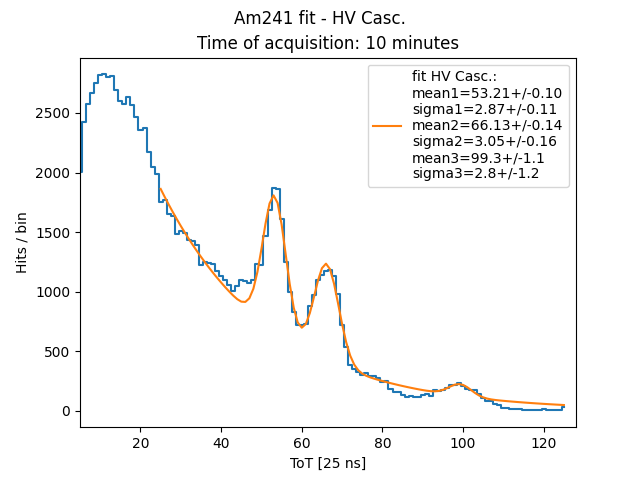
\includegraphics[scale=0.35]{am_HV Casc._peak}}\quad
\subfigure[\textbf{HV}]
{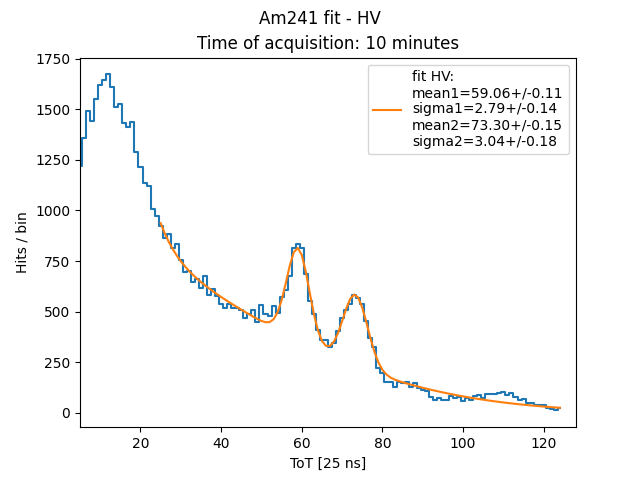
\includegraphics[scale=0.35]{am_HV_peak}}\\
\caption{\ch{^{241}Am} peaks for all frontends.}
\label{fig:am_all}
\end{figure}

%--------------------------------------------------------------------
\subsection{\ch{^{109}Cd}}

The third source employed was the \ch{^{109}Cd}. This isotope decay in \ch{^{109}Ag} by electronic capture, producing a photon of 22 KeV in the transistion. In figure \vref{cd_all} the results obtained irradiating all FE. 

\begin{figure}[h!]
\centering
\subfigure[\textbf{Normal}]
{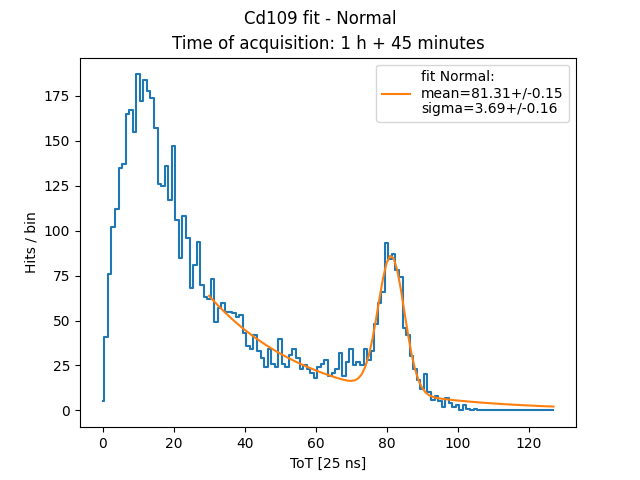
\includegraphics[scale=0.35]{cd109_Normal_peak}}\quad
\subfigure[\textbf{Cascode}]
{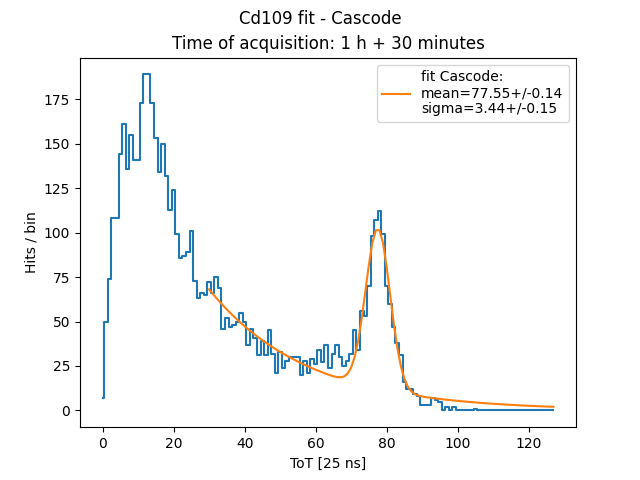
\includegraphics[scale=0.35]{cd109_Cascode_peak}}\\
\subfigure[\textbf{HV Cascode}]
{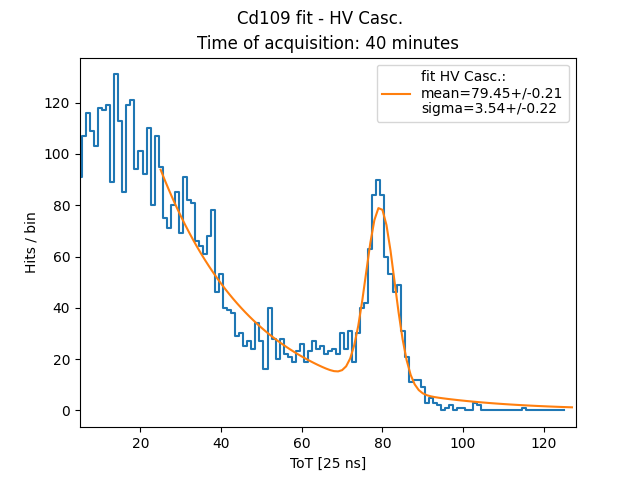
\includegraphics[scale=0.35]{cd109_HV Casc._peak}}\quad
\subfigure[\textbf{HV}]
{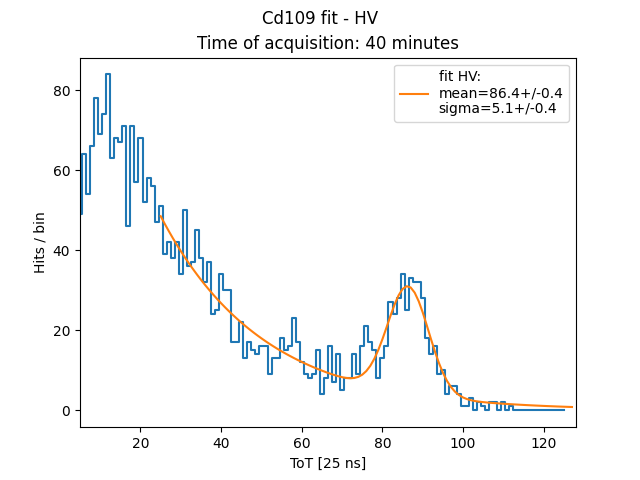
\includegraphics[scale=0.35]{cd109_HV_peak}}\\
\caption{\ch{^{109}Cd} pekas for all frontends.}
\label{fig:cd_all}
\end{figure}

%--------------------------------------------------------------------
%\subsection{\ch{^{190}Sr}}
%%apg 55 tesi


\subsection{Injection capacitance calibration}

Here it's necessary to point out that for iron source more statistics were collected so in this case a complete analysis of each pixel could be done. For the other sources instead, there weren't enough statistics on every pixel so the injection capacitance has been estimate only as a mean value for the whole front-end, just to compare with the results obtained from the iron analysis.  

In case of \ch{^{55}FE} source, we managed to fit the emission peak for each working pixel of the whole matrix. The value of the charge corresponding to the ToT peak of the emission line was extrapolate considering the parameters' values obtained by fitting the $Q_{inj}$ - ToT relationship (section \vpageref{tot_fit}). \\

Specifically the fit function \vpageref{fit_function} was inverted obtaining:

\begin{equation}
x(y) = \bigg(\frac{t}{2} - \frac{b}{2a} + \frac{y}{2a}\bigg) \pm \sqrt{\bigg(\frac{t}{2} + \frac{b}{2a} - \frac{y}{2a}\bigg)^{2} + \frac{c}{a}}
\end{equation}

where \textit{x} represents the charge corresponding to the ToT labeled by \textit{y}.

As shown in table \vpageref{tab:radio_sources}, the charge released in the sensor (considering that collected from only one pixel) corresponds roughly ($\approx$, approximately) to 1616 $e^{-}$. Therefore it was possible to calculate (estimate) the conversion factor for each pixel as follows:

\begin{equation}
C_{f}\bigg[\frac{e^{-}}{DAC}\bigg] = \frac{1616 \, e^{-}}{ToT \, \frac{DAC}{ToT unit}}
\label{inj_cap}
\end{equation} 

By these steps, a value of the injection capacitance was estimated for each well-functioning pixel. In figure \vpageref{fig:cap_dist} is reported the distributions of the injection capacitance estimated, fitted by a gaussian function.

\begin{figure}
\centering
\subfigure[\textbf{Normal}]
{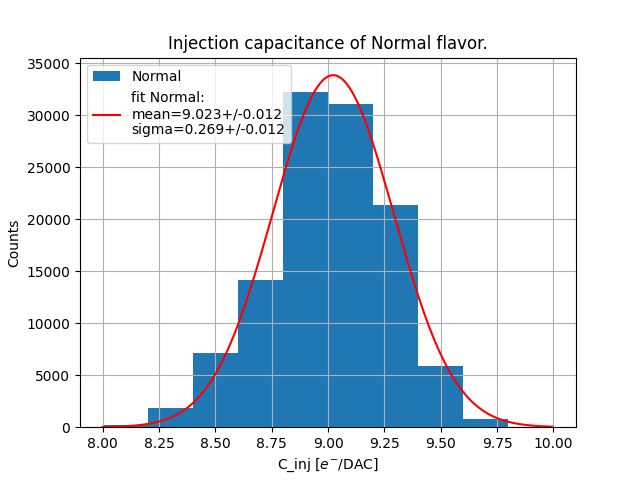
\includegraphics[scale=0.35]{c_inj_alpha_fe_Normal}}\quad
\subfigure[\textbf{Cascode}]
{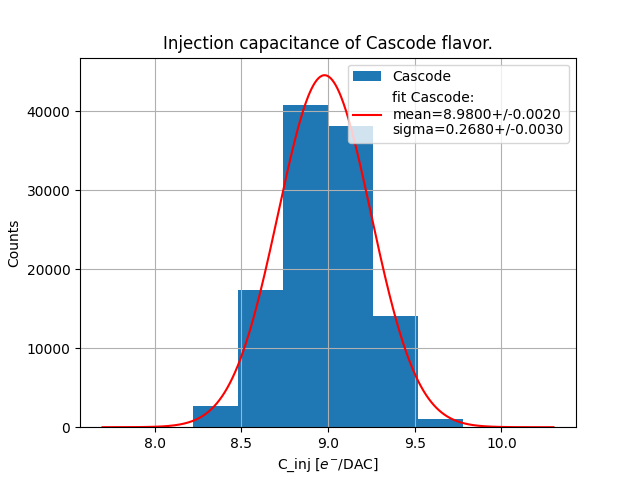
\includegraphics[scale=0.35]{c_inj_alpha_fe_Cascode}}\\
\subfigure[\textbf{HV - Cascode}]
{\includegraphics[scale=0.35]{c_inj_alpha_fe_Hv Casc.}}\quad
\subfigure[\textbf{HV}]
{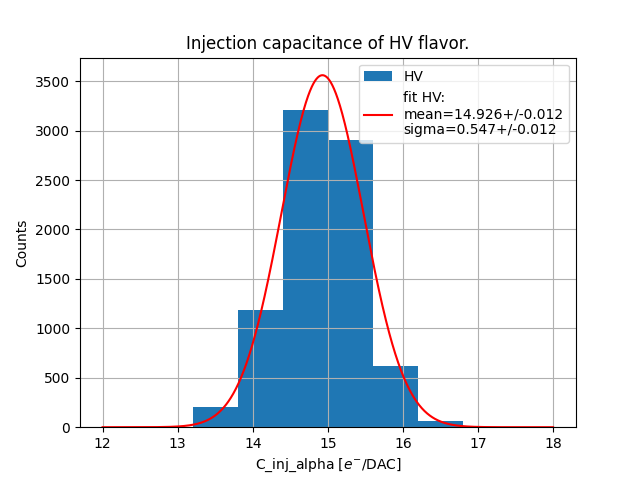
\includegraphics[scale=0.35]{c_inj_alpha_fe_HV}}\\
\caption{Injection capacitance distributions of all FE.}
\label{fig:cap_dist}
\end{figure} 

%%%%%ADD SUMMARY TABLE

[As expected the capacitance oh the HV's flavors is much higher than the Normal and Cascode FE? No! It's expected all the same?] 

Regarding the other sources, it was impossibile to fit the distributions for each pixel due to low statistics. For this reason only a mean value for all flavor could be extrapolate. In table \vpageref{tab:cap_mean} the results obtained with the same method used with the iron source, but considering all pixels of each flavor.

\begin{table}[h!]
\centering
\begin{tabular}{>{\columncolor{NavyBlue!70}} C{2.8cm}|C{1.7cm}|C{1.8cm}|C{1.7cm}|C{1.7cm}}
\rowcolor{CornflowerBlue}
Source peak & $C_{Normal}$ & $C_{Cascode}$ & $C_{HV Cascode}$ & $C_{HV}$\\[2ex]
\hline
\ch{^{55}Fe} (5.9 KeV) & 9.37 & 9.00 & 19.33 & 18.56 \\[0.5ex]
\hline
\ch{^{241}Am} (13.9 KeV) & 8.94 & 8.91 & 19.23 & 18.22 \\[0.5ex]
\hline
\ch{^{241}Am} (17.7 KeV) & 9.16 & 8.84 & 19.59 & 18.63 \\[0.5ex]
\hline
\ch{^{241}Am} (20.7 KeV) & 9.15 & 10.11 & - & -\\[0.5ex]
\hline
\ch{^{109}Cd} (22 KeV) & 9.32 & 9.39 & 20.16 & 19.6 \\[0.5ex]
\hline
\ch{^{241}Am} (26.4 KeV) & 9.60 & 9.61 & 19.25 & - \\[1.5ex]
\hline
\cellcolor{ForestGreen!80}Mean value & 9.26 & 9.31 & 19.51 & 18.75 \\[1.5ex]
\end{tabular}
\caption{Estimation of injection capacitance of all flavors for different source emission peaks.}
\label{tab:cap_mean}
\end{table}


Bringing equation \vpageref{conversion_factor} back to mind, the conversion factors of the flavors are not those expected. In particular for the HV's flavors, this factor is almost the double and it could mean that the injection capacitance is greater than expected. As matter of fact, with respect to Tj-Monopix 1, the prototype under test was design in order to have the same injection capacitance for all flavor, equal to 230 aF.

so? Loss of charge?

It's necessary to consider that maybe some measurments were dona in different conditions of pressure and temperature?

%CONTINUA%
%%Può parametrizzare perdita di segnale? viene al 51-52% non 40 come previsto.





%--------------------------------------------------------------------
\subsection{Check on linearity of tot fit}

In the end all emission peaks from the several sources have been plotted for each frontend in order to verify the agreement between their trend and the ToT-Q relationship studied by the internal injection. \\

At first the charge corresponding to the electrons expected to be released for each peaks, has been calculated with the nominal conversion factor equal to 10.1 $\frac{e^{-}}{DAC}$. As it could be seen from results in figure \vpageref{fig:inj_cap_10} there isn't good agreement between data and ToT relationship obtained(learnt) in section \vpageref{tot_fit}.


\begin{figure}
\centering
\subfigure[\textbf{Normal}]
{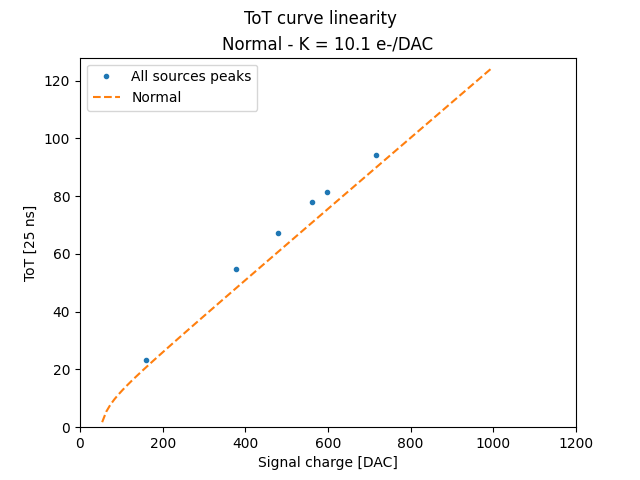
\includegraphics[scale=0.35]{ToT_Normal_thesis}}\quad
\subfigure[\textbf{Cascode}]
{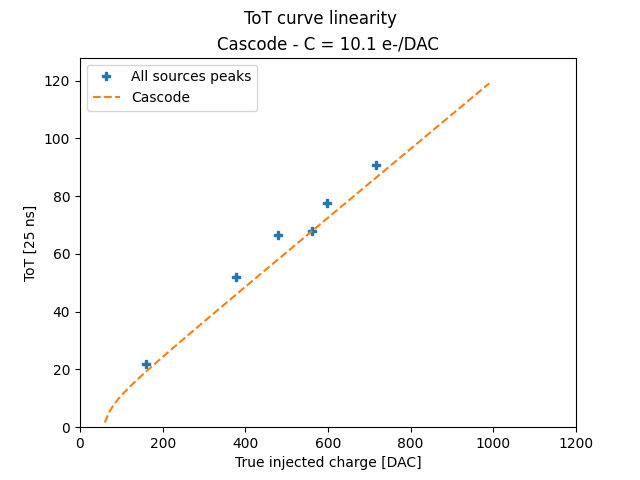
\includegraphics[scale=0.35]{ToT_Cascode_thesis}}\\
\subfigure[\textbf{HV - Cascode}]
{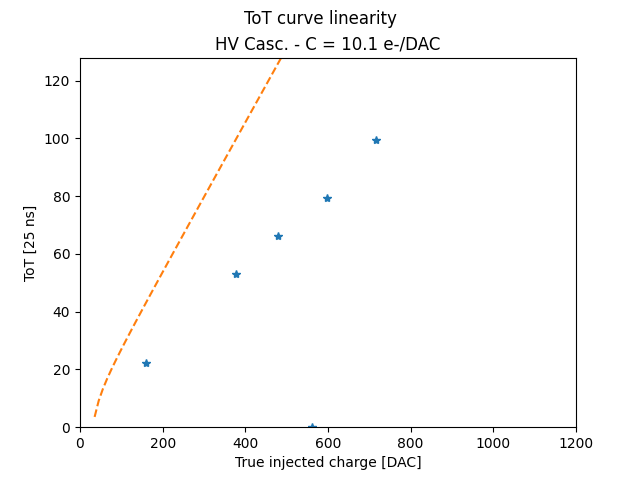
\includegraphics[scale=0.35]{ToT_HV Casc._thesis}}\quad
\subfigure[\textbf{HV}]
{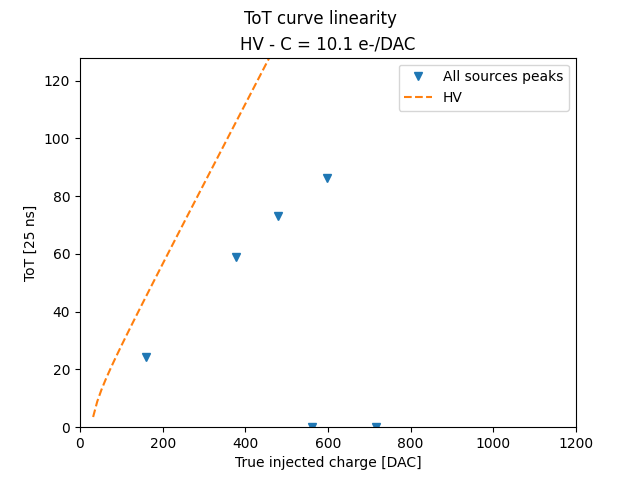
\includegraphics[scale=0.35]{ToT_HV_thesis}}\\
\caption{ToT linearity of all flavors assuming the nominal(expected) conversion factor equal to 10.1 $\frac{e^{-}}{DAC}$.}
\label{fig:inj_cap_10}
\end{figure} 

After the calibration instead, assuming the average value of injection capacitance calculated in table \vpageref{tab:}, the charge corresponding to the emission peaks have been recalculated and results are shown in figure \vpageref{fig:inj_cap_sources}.

\begin{figure}[h!]
\centering
\subfigure[\textbf{Normal}]
{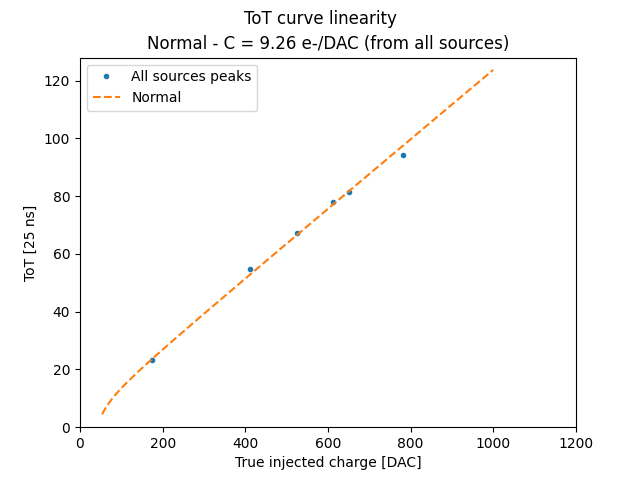
\includegraphics[scale=0.35]{ToT_Normal_sources}}\quad
\subfigure[\textbf{Cascode}]
{\includegraphics[scale=0.35]{ToT_Cascode_sources}}\\
\subfigure[\textbf{HV - Cascode}]
{\includegraphics[scale=0.35]{ToT_HV Casc._sources}}\quad
\subfigure[\textbf{HV}]
{\includegraphics[scale=0.35]{ToT_HV_sources}}\\
\caption{ToT linearity of all flavors assuming the conversion factor obtained from calibration for each FE.}
\label{fig:inj_cap_sources}
\end{figure} 

\begin{figure}[h!]
\centering
\includegraphics[scale=0.7]{Tot_linearity__sources}
\caption{Summary of trends.}
\label{inj_cap_sum}
\end{figure}

After(through) the calibration a better agreement is therefore obtained. 



%--------------------------------------------------------------------
\section{Operation with low threshold}


One of the most important target of the chip design is to keep high efficiency even after irradiation damage. All experimental environments in fact(indeed) are exposed to high doses of radiations, so it's crucial to make sure the functionality of the irradiated detectors.

For this reason, many tests were done in order to understand the chip behaviour at lower threshold that allowed to keep(mantain) good value of efficiency.
Moreover working at low threshold allowed to detect low charge events due to charge sharing or charge trapping (effect which increased after irradiation), expecially in case of thin epitaxial material. 






\begin{comment}
4. Explored also different registers settings to operate the chip with lower THResholds
 	- important after radiation damage to run at low THR to keep the hit efficiency high
5. Discovered & investigated an important issue with cross talk, due to digital signal from the redout, showing up when running the chip with THR below ~ 250 e- 
hot pixel studied to understand which digital signal was responsible & mitigate the effect with different settings/bias

Explain the function of the various registers used (see Eleonora thesis, and maybe can 		add also some scope picture). 
	Register optimization (conversion???)
	Comparison with simulation 
	Can add at the end some nice picture of the optimized thr and tuning 


boh:VOGLIAMO OPERARE A BASSE THRESHOLD PER RILEVARE EVENTI A BASSE CARICA A CAUSA DEL CHARGE TRAPPING AND CHARGE SHARING SOPRATTUTTO IN CASO DI THIN EPITAXIAL MATERIAL

\end{comment}



%--------------------------------------------------------------------
\subsection{Register optimization}

As we have seen in section (REFERENCE), there are a lot of registers which control the discriminator threshold and also the readout sequence. So preliminary it was necessary to run some tests exploring their settings in order to operate the chip at(or with) lower thresholds.\\

Now we will go through the main registers used for this purpose, in order to explain their functionality. There are several dozens of registers but we focused on some of the most important and crucial to set the threshold:

\begin{itemize}
\label{currents}
\item \textit{$I_{CASN}$} : this current is responsible of the output baseline signal[set the baseline of the FE output and change the thr] that goes to the input discriminator. In a few words, higher this value, higher the baseline, lower the threshold and also a little bit the gain. [Vice versa, decreasing this registr's value.]
\item \textit{$I_{THR}$}: it controls the pre-amplifier feedback strenght and speed, so it's responsible for the output reset rate. Increasing $I_{THR}$ results to lower gain and faster return to baseline, so higher threshold. In other words increasing this current increases the gain and the time the analog output takes to get back to the baseline and as consequence, it increase a lot the maximum value of the ToT. In fact is preferably set $I_{THR}$ to 8nA[in DAC?] in order to avoid high ToT slope.
\item \textit{$I_{DB}$}: 
\item \textit{$I_{TUNE}$}:
\item \textit{$I_{BIAS}$}: 
\item \textit{$V_{RESET}$}:  dispersion?
\end{itemize}

\begin{comment}
In section (...) some improvements of the readout with respect to TJ-Monopix 1 (analogical and digital part) have been mentioned. 
\end{comment}



%--------------------------------------------------------------------
\subsection{Comparison between data and simulation}

In the interest of understanding how the settings of the chip influence the threshold's value, several measurements have been taken varying the values of the main registers which are responsible for it.
The results are compared with simulations done by Hung Pham (...). [???]

\subsubsection{$I_{CASN}$}

This current is responsible of the output baseline. In a few words, higher this value, higher the baseline, lower the threshold and also a little bit the gain.

In figure \vref{fig:icasn_sim}, we can see the simulated behaviour of the threshold and the gain, increasing the value o $I_{CASN}$.

\begin{figure}[h!]
\centering
\includegraphics[scale=.9]{thr_gain_icasn(sim)}
\caption{Trends of Gain and Threshold increasing $I_{CASN}$.}
\label{fig:icasn_sim}
\end{figure}

To verify the trend of threshold in particular, three different acquisition have been taken by fixing $I_{THR}$ = 20, 40, 64 and increasing $I_{CASN}$ from 0  to 30 DAC, with a step of 5 DAC. We have done this enabling 200 pixels in the Cascode FE (rows: 472 - 512, cols: 225 - 230).[??]\\

The threshold distributions have been fitted with a gaussian function for each measurement,  in order to obtain the average values and their dispersion.

In figure \vref{fig:alltrends_icasn} all trends obtained from these data are reported.

[TREND OF DISPERSION?]

\begin{figure}[h!]
\centering
\includegraphics[scale=.7]{all_trends(ICASN)}
\caption{Threshold vs. $I_{CASN}$ for $I_{THR}$= 20, 40, 64.}
\label{fig:alltrends_icasn}
\end{figure}


\subsubsection{$I_{THR}$}

Reusing the same data of the previous measurements, the trend of the threshold have been studied, changing the value of $I_{THR}$ and fixing that of $I_{CASN}$. In this case only $I_{CASN}$ from 0 to 15 DAC is considered, because for higher values we don't have enough measures of the threshold (specifically only two for $I_{THR}$=40, 64). The results are shown in figure \vref{fig:alltrends_ithr}.

\begin{figure}[h!]
\centering
\includegraphics[scale=.7]{all_trends(ITHR)}
\caption{Threshold vs. $I_{THR}$ for $I_{CASN}$= 0, 5, 10, 15.}
\label{fig:alltrends_ithr}
\end{figure}

We can compare them with the simulation done by Hung Pham in figure \vref{fig:ithr_sim}. 

\begin{figure}[h!]
\centering
\includegraphics[scale=.7]{ithr_simulation}
\caption{Trends of Gain and Threshold increasing $I_{CASN}$.}
\label{fig:ithr_sim}
\end{figure}



\subsubsection{Time over Threshold (ToT)}

The last analysis done in order to make a comparison with the simulations, is about the trend of the ToT changing the value of $I_{CASN}$ for a fixed value of $I_{THR}$ and vice versa. In particular we consider the data obtained with $I_{CASN}$ fixed to 0 DAC and $I_{THR}$ to 64 DAC, which are the values studied and used for this registers during the Test Beam in Desy.

\begin{figure}[h!]
\centering
\subfigure[ToT vs $I_{THR}$ ($I_{CASN}$=0 DAC) - Data (\textbf{Cascode})]
{\includegraphics[scale=0.45]{tot_curves_icasn0}}\quad
\subfigure[ToT vs $I_{THR}$ ($I_{CASN}$=0 DAC) - Simulation]
{\includegraphics[scale=0.5]{tot_curves_icasn0_simu}}\\
\caption{ToT vs $I_{THR}$}
\label{fig:tot_vs_ithr}
\end{figure}

\begin{figure}[h!]
\centering
\subfigure[ToT vs $I_{CASN}$ ($I_{THR}$=64 DAC) - Data (\textbf{Cascode})]
{\includegraphics[scale=0.5]{tot_curves_ithr64}}\\%\quad
\subfigure[ToT vs $I_{CASN}$ ($I_{THR}$=64 DAC) - Simulation]
{\includegraphics[scale=0.35]{tot_curves_ithr64_simu}}\\
\caption{ToT vs $I_{CASN}$}
\label{fig:tot_vs_icasn}
\end{figure}


%--------------------------------------------------------------------
\subsubsection{some nice picture of the optimized thr and tuning}


!!!!!!!!!!!!!!!!!!!!!!!!!!!!!




\section{Cross talk issue and mitigation}

As it was already pointed out, during the measurements of the average threshold of all FE (section REFERENCE), there were something atypical in the s-curves of the HVs flavor, because some of pixels seem to have occupancy greater than 1. This behavior threatens the good functionality of the overall matrix response, because some pixels flood the readout, giving floating results.(all readout process)\\

Also during the systematic study of the main registers' values, the presence of the hot pixels has prevented to use certain settings and as consequence to reach lower global thresholds. 

For this reason an investigation has been conducted in order to understand the reasons why and to cure them as far as possible.
During this study an important issue with cross-talk(readout signal) was discovered, and so in this section we examine this effect and some attempts(tries) to mitigate it using different settings/bias.


\subsection{Hot pixel issue}

First of all we noticed that in the s-curves oh the HVs flavor, for example that of HV-Cascode in figure \vpageref{fig:hot_first}, the atypical behavior could be triggered by a digital signal sent to the matrix during the readout activity at low threshold, for two main reasons:

\begin{itemize}
\item when the matrix has high threshold, like for Normal and Cascode FE, all pixels seem to behave as expected.\\ Lowering the threshold and running some source acquisitions without any source no strange behaviour was observed. Acquiring data with a radioactive source instead, even Normal and Cascode FE seem to reveal the same problem. This led to thinking that during the readout of good pixels an induced signal is created which couples with some other pixels, in particular with those at lower threshold with respect to the average value. If the hejght of this signal exceed the threshold of the single pixel, it causes some spurious hits, making the pixel ''\textbf{hot}''.

\item Moreover, considering the HV Cascode s-curves, it could be noticed that in the region before the threshold (($Q_{inj}$<threshold,pointed by the blue arrow) there isn't an anomalous activity which means tha the induced signal is not due to the BCID tha is always sent to the matrix during the injection or an acquisition with the source, regardless of being above or below the  threshold. The atypical behaviour indeed, is in the region above the threshold ($Q_{inj}$>threshold, pointed by the red arrow) where the occupancy of some pixels becomes greater than 1. This means that these \textit{hot pixels} detect more hits of those injected.

\end{itemize} 

\begin{figure}[h!]
\centering
\includegraphics[scale=.5]{hot_first_HV}
\caption{HV-Cascode s-curves.}
\label{hot_first}
\end{figure}

From these first observations, we have reached the conclusion that the cross talk could be tied to the readout activity. So we have started investigating the timestamp of the hits (out of synch) not synchronize with the timestamp of the injection.


\subsection{Hot pixel strategy (study)}

At first, it has been lowered the threshold in order to ''create'' hot pixel also in the first two flavors of the matrix. In fact with TB settings the threshold was too high and the hypothetical induced signal didn't caused sporious hits. For this purpose ( to this end, to do this) different settings were tried, changing some fundamental registers responsible for the threshold like those listed and explained \vpageref{currents}. 

Then it was tried to run tests under controlled conditions:
\begin{itemize}
\item one healty(good) pixel was injected;
\item one \textit{hot pixel} (or two or three in next test) was enabled but not injected;
\item the all matrix except these pixels was disabled.
\end{itemize}

In this way (thus) (remembering the readout sequence [REFERENCE]) the readout cycle had a known duration and two timing info and some precautions had been be used to study the induced signal with greater precision:

\begin{itemize}
\item \textbf{$\Delta$TS} (TimeStamp) between two consecutive hits: the TimeStamp is assigned from the FPGA when the \textsc{token} rises on the TE of the first hit to read, but only if the previous readout frame is completed. So, if the hit coming from a \textit{hot pixel} is after the hit from the injected one, the minimum $\Delta TS$ has to be equal to the readout time of 1 pixel and so the duration (period) of the signal \textsc{FREEZE\_STOP}.\\
This info has allowed to verify if the hot pixel fires after the good injected one or not.
\item LE(hit) - TE(previous hit): this quantity measures the elapsed time between a hit and the previous one. This is a finer ingo than the $\Delta$TS because it allows to correlate the hit with the induced digital signal, originate from the readout cycle.
\end{itemize}

Moreover, since a 7-bit BCID is sent to the matrix during its activity, it was important to keep short (<128 clock cycle) the duration of the full readout sequence and to not enable too many pixels in order to not extend too much the readout frame. Otherwise the information on the leading edge of the pixel could not be correlated with the token of the previous hit. In other words, if the readout frame exceed 128 clock cycles, since the token could be raised if the matrix is \textbf{not} freeze, even if an hit is arrived before it could be read only in the next frame when it could rise again the token, but in this case it will have different TimeStamp. So in this case the TS is useless for our purpose.


\subsection{Cross-talk (Results)}

Referring to the readout sequence explained in section [REFERENCE], in order to understand which signal could induced cross talk, each register's value has been moved one by one.
In table \vpageref{tab:ro_registers} just an example of the seravl settings tried.

\begin{table}[h!]
\centering
\begin{tabular}{>{\columncolor{ForestGreen!60}} C{5cm}|C{1.7cm}}
\rowcolor{PineGreen!80}
Register & Value \\
\hline
\textsc{FREEZE\_START\_CONF} & 10\\[0.3ex]
\hline
\textsc{READ\_START\_CONF}& 13 \\[0.3ex]
\hline
\textsc{READ\_STOP\_CONF} & 15 \\[0.3ex]
\hline
\textsc{LOAD\_CONF} & 30 \\[0.3ex]
\hline
\textsc{FREEZE\_STOP\_CONF} & 31\\[0.3ex]
\hline
\textsc{STOP\_CONF} & 31\\[0.3ex]
\hline
\end{tabular}
\caption{Registers of the Readout cycle.}
\label{tab:ro_registers}
\end{table}

Doing so indeed, the LE-TE info has to shift by the same value, in correspondence with the signal that cause the cross talk. This step of the procedure is tied with the necessity to keep the readout sequence within the maximum 128 BCID range.\\

For example, if \textsc{FREEZE\_START\_CONF} is responsible for the cross talk signal, shifting is value by a certain amount, we expcted that the hot pixels start to fire after that this signal arises due to the hit on the injected pixel. So the value of LE-TE has to be \textsc{FREEZE\_START\_CONF} + some potential(possible, probable) delay. Same argument for the other registers. \\

By this procedure, repeated for each readout register, we have come to the conclusion that the cross-talk could be related to the raising and falling edge of the \textsc{FREEZE} signal.

In figure \vpageref{fig:xtalk} an example of some results obtained. It is the histogram of the time last between the leading edge of an hit and the trailing edge of the previous hit, when one pixel is injected and two are read. It's possible to see several peaks (reffering to the readout setting reported in table \vpageref{tab:ro_registers}):

\begin{itemize}
\item one at 0, that represent the situation in which both hits come from hot pixel firing simultanously after the injection. This means that they are activated by the same signal and so is the most important confirmation that is cross-talk and not random firing pixel signal;
\item one at $\approx$ 18 equal to \textsc{FREEZE STAR} raising + 8 $\rightarrow$ first induced signal;
\item one at $\approx$ 35 equal to \textsc{FREEZE STOP} falling + 4 $\rightarrow$ second induced signal;
\item one at $\approx$ 55 equal to \textsc{FREEZE STOP} falling + 4 when two different pixels are read (specifically in this case after the first 30 time unit until the \textsc{LOAD CONF}, a distinct pixel reading starts and it last another 20 time unit (\textsc{LOAD} - \textsc{FREEZE START}) + 1 unit time to conclude the frame with the \textsc{FREEZE STOP} and so 51 + 4 unit time wrote above. So when two pixels are read, the \textsc{FREEZE STOP} falling after 51 clock cycles, and it is compatible with the last peak in the plot.
\end{itemize}

%%ReFIRING???

\begin{figure}[h!]
\centering
\subfigure[An example of the time quantity used in the analysis.]
{\includegraphics[scale=0.8]{xtalk_time}}\quad
\subfigure[An example of the LE(hit)-TE(previous hit) histogram.]
{\includegraphics[scale=0.4]{xtalk_hist}}\\
\caption{Some results of the cross-talk studies.}
\label{fig:xtalk}
\end{figure}

As already stated, we run several tests varying the number of pixels to read, the value of the readout registers, different combination of hot and good pixels and also different spatial location of them in the matrix to exclude the possibility that the problem was related to particular columns. All results are in agreement with the interpretation explained above.\\

MAH...\\
Furthermore it hase been tried to estimate the height of the induced signal from the threshold of the hot pixel. For this reason we have have tried different setting of the currents cited above to make a pixel \textit{hot} in order to understand when the induced signal went above the threshold. We have found that the signal could (may) correspond to 100/150 $e^{-}$.\\

%the height of the cross talk signal from FREEZE was measured lowering gradually the THR of good pixels to monito when they become hot.

In figure \vpageref{fig:analog_xtalk} an analog acquistion of the readout signals taken by an oscilloscope.


\begin{figure}
\centering
\includegraphics[scale=.6]{xtalk_analog}
\caption{Cross-talk of the \textsc{FREEZE} signal on oscilloscope's analog output, for different value of \textsc{FREEZE\_START\_CONF} register.}
\label{fig:analog_xtalk}
\end{figure}

In these tests one pixel was injected from 0 to 140 DAC (in the acquisition it can be seen in the increasing signal height). There are two different group of spikes, the first which smaller and represent the cross-talk from the raising of the \textsc{FREEZE} signal and the second, larger and corresponding to the cross talk from the falling edge of the same signal.
Moreover it's possible to see that in the two different pictures, the cross talk signals move according to the different settings of the \textsc{FREEZE START/STOP} edge.

%meglio una lista??


\subsection{Mitigation}

As seen in the previous, the problem of the hot pixel is tied to the induction signal produced during the readout which cause cross-talk. It becomes more important(significant, serious) when there is grater dispersion threshold.\\

Potentially every pixel could become \textit{hot} if its threshold is lower than the height of the cross-talk signal since the \textsc{FREEZE} in sent across the entire matrix. 

As an example in figure \vpageref{making_hot} it si possible to compare the behaviour of pixel (218, 123) changing(modifying) some registers' values in order to reduce the threshold.

\begin{figure}[h!]
\centering
\subfigure[$I_{DB}$=100, $I_{TUNE}$=53 - Good behavior]
{\includegraphics[scale=0.35]{making_hot1}}\quad
\subfigure[$I_{DB}$=60, $I_{TUNE}$=150 - Pixel starts to misbehave]
{\includegraphics[scale=0.35]{making_hot3}}\\
\subfigure[$I_{DB}$=55, $I_{TUNE}$=150 - Pixel becomes \textit{hot}]
{\includegraphics[scale=0.35]{making_hot2}}\\
\caption{S-curve of the pixel (218, 123) for different register settings.}
\label{fig:making_hot}
\end{figure}

 
For this reason, a possible treatment could be related to the threshold tuning, explained in section (reference) , which could allow to make the pixesl threshold more uniform (less threshold dispersion) and simultanously targeting a value greater than the induced signals. \\

In figure \vpageref{fig:tuning_hot} an example of the results obtained.

\begin{figure}
\centering
\subfigure[Threshold distribution before tuning procedure.]
{\includegraphics[scale=0.3]{before_tuning}}\quad
\subfigure[Threshold distribution after tuning procedure.]
{\includegraphics[scale=0.3]{after_tuning}}\\
\caption{Threshold tuning to reduce hot pixels.}
\label{fig:tuning_hot}
\end{figure} 

It' evident the reduction of the tail in the threshold distribution, in fact the dispersion is reduced by 56\%. Also the hot pixels decrease from 18\% to 1.2\% of the total number of pixels studied. [We can noticed indeed that the peak at 0 threshold disappears.]

%It was effectively done managing to obtin lower threshold
%DEVI METTERE ESEMPIO???
%DAC tuning kaje threshold more uniform, threat hot pixel and so also the peak at zero tot in source acquisition is reduced

Moreover it has been tried to increase the voltage bias of the all matrix, too. We remember that all previous test has been run with $P_{WELL}/P_{SUB}$ set to -3 V. This value was increased to -6 V and indeed there were some improvements. In fact increasing the bias, we expected a decrease of the diode capacitance thus higher gain and lower thresold dispersion. In addition the coupling with the cross talk signal is reduced too and so the induced signal height. \\
In figure \vpageref{fig:bias_comp} a comparison between the threshold distribution respectively at -3 V and -6 V, with same registers setting and without tuning.

\begin{figure}[h!]
\centering
\subfigure[Threshold distibution at $P_{WELL}/P_{SUB}$=-3 V.]
{\includegraphics[scale=0.3]{th_dist_3V}}\quad
\subfigure[Threshold distibution at $P_{WELL}/P_{SUB}$=-6 V.]
{\includegraphics[scale=0.3]{th_dist_6V}}\\
%\caption{}
\label{fig:bias_comp}
\end{figure}

At higher bias voltage not only is the threshold lower (higher gain), but also its dispersion, as expected. And despite that there are fewer hot pixels: 1.3\% at -6V against 17\% at -3 V. Also here it's clear a reduction of the threshold distribution tail. 

\subsubsection{Final results?}

Eventually the final results obtained with both threshold tuning and a bias voltage on $P_{WELL}/P_{SUB}$=-6 V. 

\begin{figure}[h!]
\centering
\subfigure[Threshold distibution at $P_{WELL}/P_{SUB}$=-6 V without tuning.]
{\includegraphics[scale=0.3]{xtalk_6V_no_tuning}}\quad
\subfigure[Threshold distibution at $P_{WELL}/P_{SUB}$=-6 V with tuning.]
{\includegraphics[scale=0.3]{xtalk_6V_tuning}}\\
%\caption{}
\label{fig:bias_tuning}
\end{figure}

As we can see in figure \vpageref{fig:bias_tuning}, the threshold dispersion decreases with the number of hot pixels. In fact without tuning there are 1.3\% of them, instead with tuning procedure there are none at all.



%LOWERING ITHR DECREASED THE INDUCED SIGNAL, BUT MATRIX NOT GOOD FUNCTIONALITY?
%VRESET(agisce sulla dispersione) AND IBIAS(aumenta gain e diminuisce dispersion ma aumenta power consumption)



\begin{comment}
Suggestions from OBELIX meeting.

Probably the coupling is linked to digital power. 
Not from the bulk: +4 clk seems to be the indication for not a direct coupling

Since the distribution of the power is from the edge,  first and last column should be more solid against this effect and hot pixel should be more present in the center? 
They asked if we have a  map of the hot pixels

Also suggested to change the clock and see if the delay from the FREEZE edge is at the same delay or not. 

\end{comment}



%%%%%%%%%%%%%%%%%%%%%%%%%%%%%%%%%%%%%%%
%%%%%%%%%%%%%%%%%%%%%%%%%%%%%%%%%%%%%%%

%\subsection{Readout sequence}    %NEL QUARTO

%%%%%%%%%%%%%%%%%%%%%%%%%%%%%%%%%%%%%%%
%%%%%%%%%%%%%%%%%%%%%%%%%%%%%%%%%%%%%%%





\section{Test Beam results}

Hit detection efficiency from bespin article

\begin{comment}
So with this test we have fully characterized the main features of the chip W14R12, which are then used to interpret data from Test Beam in June 2022 in Desy.

In the following some of the results obtained:
\end{comment}












































%%%%%%%%%%%%%%%%%%%%%%%%%%%%%%
%			COMMENT						
%%%%%%%%%%%%%%%%%%%%%%%%%%%%%%

\begin{comment}

The ultimate purpose of this measurement is to describe (characterize) the response of each pixel by injecting a charge equivalent to the typical energy released from particles emitted in decays of radioactive materials. As explained in the previous section (reference), for example the \ch{^{55}Fe} has an emission spectrum with quite sharp lines and this allows to compare data more easily. The first line is at 5.9 KeV which corresponds on average to about 1616 $e^{-}$ released (through the pixel??).

\begin{figure}[h!]
\centering
\includegraphics[scale=0.8]{spectrum_fe}
\caption{\ch{^{55}Fe} (radioactive source) emission spectrum using the analog output of a PMOS reset front-end of TJ-Monopix 1. (reference)}
\label{fig:fespectrum}
\end{figure}

\end{comment}

\begin{comment}
\subsubsection{$V_{CASP}$}

[Explain VCASP]

In order to enhance this type of analysis, other scans have been run increasing the value of $V_{CASP}$ from 3 to 143, with a step of 10 DAC unit. In figure \vref{fig:th_vs_casp} the threshold's trend with respect to different values of this register.

\begin{figure}[h!]
\centering
\includegraphics[scale=.7]{TH_vs_VCASP(point)}
\caption{Trends of Threshold increasing $V_{CASP}$.}
\label{fig:th_vs_casp}
\end{figure}
\end{comment}


\begin{comment}
\begin{figure}[h!]
\centering
\subfigure[VH = 140 DAC]
{\includegraphics[scale=0.6]{all_norm_thdist_140}}\quad
\subfigure[VH = 200 DAC]
{\includegraphics[scale=0.6]{all_norm_thdist_200}}\\
\caption{Threshold distributions of \textbf{Normal} flavor before and at the maximum saturation, respectively.}
\label{fig:thdist_norm}
\end{figure}

\begin{figure}[h!]
\centering
\subfigure[VH = 140 DAC]
{\includegraphics[scale=0.5]{all_casc_thdist_140}}\quad
\subfigure[VH = 200 DAC]
{\includegraphics[scale=0.5]{all_casc_thdist_200}}\\
\caption{Threshold distributions of \textbf{Cascode} flavor before and at the maximum saturation, respectively.}
\label{fig:thdist_casc}
\end{figure}

\begin{figure}[h!]
\centering
\subfigure[VH = 140 DAC]
{\includegraphics[scale=0.5]{all_HVc_thdist_140}}\quad
\subfigure[VH = 200 DAC]
{\includegraphics[scale=0.5]{all_HVc_thdist_200}}\\
\caption{Threshold distributions of \textbf{HV Cascode} flavor before and at the maximum saturation, respectively.}
\label{fig:thdist_hvc}
\end{figure}

\begin{figure}[h!]
\centering
\subfigure[VH = 140 DAC]
{\includegraphics[scale=0.5]{all_HV_thdist_140}}\quad
\subfigure[VH = 200 DAC]
{\includegraphics[scale=0.5]{all_HV_thdist_200}}\\
\caption{Threshold distributions of \textbf{HV} flavor before and at the maximum saturation, respectively.}
\label{fig:thdist_hvc}
\end{figure}
\end{comment}

%----------------------------------------------------------------------------------------------------


\begin{comment}
For the greater (higher) injection height, 8 different measurement have be actually done, each one on 28 consecutive columns and on all rows. Then data have been put together to obtain a single (summary) plot on the whole flavor. Same procedure has been preformed on the \textbf{Cascode FE}.
\end{comment}

\begin{comment}


%\subsection{Measurement of the average threshold shift for injected charge greater than 140 DAC}

To evaluate this artificial shift of the threshold, two different measurements have been done for each flavor:

\begin{itemize}
\item for an injected charge equal to 140 DAC $\rightarrow$ before the saturation region;
\item for an injected charge equal to 200 DAC $\rightarrow$ almost the maximum limit of the saturation region (from this value onward only the threshold increases, not the injected charge).
\end{itemize}

The threshold distributions obtained from each measurements have been fitted to extract an average value on the whole flavor. Naming $Q_{th, 140}$ and $Q_{th, 200}$  the threshold obtained from injections of 140 and 200 DAC respectively, the mean shift has been estimated by:

\begin{equation}
\Delta Q = Q_{th,200} - Q_{th,140}
\end{equation}

Eventually, this charge shift has been subtracted from data collected for an injection pulses of 200 DAC, in order to extrapolate the response in ToT of the injected pixels up to a value of 170 DAC.

What has been obtained is reported in the following section, together with a briefly explanation of the method used to evaluate the threshold.

\end{comment}

\begin{comment}

\begin{table}[h!]
\centering
\begin{tabular}{>{\columncolor{ProcessBlue!60}} C{3.5cm}|C{3.5cm}}
\rowcolor{lightgray}
Registri & Default Settings (''GOE'') [DAC unit]\\[2ex]
\hline
$I_{THR}$ & 64 \\[0.5ex]
\hline
$I_{BIAS}$ & 50 \\
\hline
$V_{RESET}$ & 143 \\
\hline
$I_{CASN}$ & 0 \\
\hline
$V_{CASP}$ & 93 \\
\hline
$V_{CASC}$ & 228 \\
\hline
$I_{DB}$ & 100 \\
\hline
$I_{TUNE}$ & 53 \\
\hline
$V_{CLIP}$ & 255 \\
\hline
$I_{COMP}$ & 80 \\
\hline
$I_{DEL}$ & 88 \\
\hline
$I_{RAM}$ & 50 \\
\hline
\end{tabular}
\caption{Settings of the main registers used for the W14R12 chip, for Normal and Cascode flavors, during the Test Beam in Desy.}
\label{tab:tb_settings}
\end{table}

\begin{table}[h!]
\centering
\begin{tabular}{>{\columncolor{Green!60}} C{3.5cm}|C{3.5cm}}
\rowcolor{lightgray}
Registri & Default Settings (''GOE'') [DAC unit]\\
\hline
$I_{THR}$ & 30 \\
\hline
$I_{BIAS}$ & 60 \\
\hline
$V_{RESET}$ & 100 \\
\hline
$I_{CASN}$ & 8 \\
\hline
$V_{CASP}$ & 40 \\
\hline
$V_{CASC}$ & 228 \\
\hline
$I_{DB}$ & 100 \\
\hline
$I_{TUNE}$ & 53 \\
\hline
$V_{CLIP}$ & 255 \\
\hline
$I_{COMP}$ & 80 \\
\hline
$I_{DEL}$ & 88 \\
\hline
$I_{RAM}$ & 50 \\
\hline
\end{tabular}
\caption{Settings of the main registers used for the W14R12 chip, for the HV's flavors, during the Test Beam in Desy.}
\label{tab:tb_hv_settings}
\end{table}
\end{comment}

\begin{comment}
\begin{figure}[h!]
\centering
\includegraphics[scale=0.5]{all_HV_thdist_140}
\caption{Threshold distributions of \textbf{HV} flavor for VH = 140 DAC}
\label{fig:thdist_hv}
\end{figure}
\end{comment}

\begin{comment}
\begin{figure}[h!]
\centering
\includegraphics[scale=0.5]{all_norm_thdist_140}
\caption{Threshold distributions of \textbf{Normal} flavor for VH = 140 DAC}
\label{fig:thdist_norm}
\end{figure}
\end{comment}

\begin{comment}
\begin{figure}[h!]
\centering
\includegraphics[scale=0.5]{all_casc_thdist_140}
\caption{Threshold distributions of \textbf{Cascode} flavor for VH = 140 DAC.}
\label{fig:thdist_casc}
\end{figure}
\end{comment}

\begin{comment}
\begin{figure}[h!]
\centering
\includegraphics[scale=.5]{all_HVc_thdist_140}
\caption{Threshold distributions of \textbf{HV Cascode} flavor for VH = 140 DAC.}
\label{fig:thdist_hvc}
\end{figure}
\end{comment}

\begin{comment}
In the last plots of this section (\vpageref{fig:tot_vs_vcasp}) are reported the trends of the ToT varying the value of $V_{CASP}$ for both Normal and Cascode FE, but there aren't simulations to make a comparison. 

\begin{figure}[h!]
\centering
\subfigure[ToT vs $V_{CASP}$ - Data (\textbf{Cascode})]
{\includegraphics[scale=0.4]{tot_vcasp(cascode)}}\quad
\subfigure[ToT vs $V_{CASP}$ - Data (\textbf{Normal})]
{\includegraphics[scale=0.4]{tot_vcasp(normal)}}\\
\caption{ToT vs $V_{CASP}$}
\label{fig:tot_vs_vcasp}
\end{figure}
\end{comment}


\begin{comment}
\begin{itemize}
\item[$I_{THR}=64$]:

\begin{tabular}{c | c | c}
$I_{CASN}$ [DAC] & THR [DAC] & THR Dispersion [DAC]\\
\hline
0 & 61.43 & 2.45\\
5 & 53.42 & 2.45\\
10 & 50.33 & 2.45\\
15 & 48.21 & 2.41\\
20 & 46.70 & 2.38\\
25 & 45.49 & 2.52\\
30 & 46.09 & 2.50
\end{tabular}

\item[$I_{THR}=40$]:

\begin{tabular}{c | c | c}
$I_{CASN}$ [DAC] & THR [DAC] & THR Dispersion [DAC]\\
\hline
0 & 47.28 & 2.12\\
5 & 41.07 & 2.02\\
10 & 38.39 & 2.03\\
15 & 36.65 & 1.95\\
20 & 35.53 & 1.91\\
25 & NaN & NaN\\
30 & 33.37 & 2.04
\end{tabular}

[Here we can see a particular setting, that is $I_{THR}=40$ AND $I_{CASN}$=25, for which the chip doesn't seem to work.
PIXEL THAT FIRE UP??]

\item[$I_{THR}=20$]:

\begin{tabular}{c | c | c}
$I_{CASN}$ [DAC] & THR [DAC] & THR Dispersion [DAC]\\
\hline
0 & 34.43 & 1.95\\
5 & 28.10& 1.72\\
10 & 26.59 & 1.75\\
15 & 24.66 & 1.77\\
\end{tabular}
\medskip\\

\end{itemize}
\end{comment}

\begin{comment}
During this study an iportant issue with cross-talk(readout signal) was discovered. As it was already mentioned, also in the threshold analysis for the HVs flavors, there were something atypical in the s-curves, because some of them seem to have occupancy greater than 1!
So in this section we will go through this effect and some attempt to mitigate the effect using different settings/bias. 

\end{comment}



%%%%%%%%%%%%%%%%%%%%%%%%%%
%			BIBLIOGRPAHY
%%%%%%%%%%%%%%%%%%%%%%%%%%

%1. THESIS MUSTAKAS
%2. GAMMA RAY SPECTRUM OF AM-241 IN A BACK SCATTERING GEOMETRY USING A HIGH PURITY GERMANIUM DETECTOR (for Am241) 
%KOLANOSKI per converision factro 3.65
% slide degli altri da vtx meeting
%ALTRE TESI?
%CDR
%articoli giuliana
